%==========================================
%
% SIBGRAPI 2024 paper template
% Example of IEEEtran.cls
%
%==========================================

% *** Authors should verify (and, if needed, correct) their LaTeX system  ***
% *** with the testflow diagnostic prior to trusting their LaTeX platform ***
% *** with production work. The IEEE's font choices and paper sizes can   ***
% *** trigger bugs that do not appear when using other class files.       ***                          ***
% The testflow support page is at:
% http://www.michaelshell.org/tex/testflow/

\documentclass[10pt,conference]{IEEEtran}


% Some very useful LaTeX packages include:
% (uncomment the ones you want to load)


% *** MISC UTILITY PACKAGES ***
%
%\usepackage{ifpdf}
% Heiko Oberdiek's ifpdf.sty is very useful if you need conditional
% compilation based on whether the output is pdf or dvi.
% usage:
% \ifpdf
%   % pdf code
% \else
%   % dvi code
% \fi
% The latest version of ifpdf.sty can be obtained from:
% http://www.ctan.org/pkg/ifpdf
% Also, note that IEEEtran.cls V1.7 and later provides a builtin
% \ifCLASSINFOpdf conditional that works the same way.
% When switching from latex to pdflatex and vice-versa, the compiler may
% have to be run twice to clear warning/error messages.






% *** CITATION PACKAGES ***
%
\usepackage{cite}
% cite.sty was written by Donald Arseneau
% V1.6 and later of IEEEtran pre-defines the format of the cite.sty package
% \cite{} output to follow that of the IEEE. Loading the cite package will
% result in citation numbers being automatically sorted and properly
% "compressed/ranged". e.g., [1], [9], [2], [7], [5], [6] without using
% cite.sty will become [1], [2], [5]--[7], [9] using cite.sty. cite.sty's
% \cite will automatically add leading space, if needed. Use cite.sty's
% noadjust option (cite.sty V3.8 and later) if you want to turn this off
% such as if a citation ever needs to be enclosed in parenthesis.
% cite.sty is already installed on most LaTeX systems. Be sure and use
% version 5.0 (2009-03-20) and later if using hyperref.sty.
% The latest version can be obtained at:
% http://www.ctan.org/pkg/cite
% The documentation is contained in the cite.sty file itself.


%\usepackage{svg}




% *** GRAPHICS RELATED PACKAGES ***
%
\ifCLASSINFOpdf
   \usepackage[pdftex]{graphicx}
  % declare the path(s) where your graphic files are
   \graphicspath{{figs/}}
  % and their extensions so you won't have to specify these with
  % every instance of \includegraphics
   \DeclareGraphicsExtensions{.pdf,.jpeg,.png}
\else
  % or other class option (dvipsone, dvipdf, if not using dvips). graphicx
  % will default to the driver specified in the system graphics.cfg if no
  % driver is specified.
   \usepackage[dvips]{graphicx}
  % declare the path(s) where your graphic files are
   \graphicspath{{../figs/}}
  % and their extensions so you won't have to specify these with
  % every instance of \includegraphics
   \DeclareGraphicsExtensions{.eps}
\fi
% graphicx was written by David Carlisle and Sebastian Rahtz. It is
% required if you want graphics, photos, etc. graphicx.sty is already
% installed on most LaTeX systems. The latest version and documentation
% can be obtained at: 
% http://www.ctan.org/pkg/graphicx
% Another good source of documentation is "Using Imported Graphics in
% LaTeX2e" by Keith Reckdahl which can be found at:
% http://www.ctan.org/pkg/epslatex
%
% latex, and pdflatex in dvi mode, support graphics in encapsulated
% postscript (.eps) format. pdflatex in pdf mode supports graphics
% in .pdf, .jpeg, .png and .mps (metapost) formats. Users should ensure
% that all non-photo figures use a vector format (.eps, .pdf, .mps) and
% not a bitmapped formats (.jpeg, .png). The IEEE frowns on bitmapped formats
% which can result in "jaggedy"/blurry rendering of lines and letters as
% well as large increases in file sizes.
%
% You can find documentation about the pdfTeX application at:
% http://www.tug.org/applications/pdftex





% *** MATH PACKAGES ***
%
\usepackage[cmex10]{amsmath}
% A popular package from the American Mathematical Society that provides
% many useful and powerful commands for dealing with mathematics.
%
% Note that the amsmath package sets \interdisplaylinepenalty to 10000
% thus preventing page breaks from occurring within multiline equations. Use:
\interdisplaylinepenalty=2500
% after loading amsmath to restore such page breaks as IEEEtran.cls normally
% does. amsmath.sty is already installed on most LaTeX systems. The latest
% version and documentation can be obtained at:
% http://www.ctan.org/pkg/amsmath
\usepackage{amsmath,amssymb,amsfonts}
\newtheorem{definition}{Definition}


\usepackage{tabularx, booktabs}

\usepackage[english, englishkw,  ruled, linesnumbered]{algorithm2e}


% *** SPECIALIZED LIST PACKAGES ***
%
%\usepackage{algorithmic}
% algorithmic.sty was written by Peter Williams and Rogerio Brito.
% This package provides an algorithmic environment fo describing algorithms.
% You can use the algorithmic environment in-text or within a figure
% environment to provide for a floating algorithm. Do NOT use the algorithm
% floating environment provided by algorithm.sty (by the same authors) or
% algorithm2e.sty (by Christophe Fiorio) as the IEEE does not use dedicated
% algorithm float types and packages that provide these will not provide
% correct IEEE style captions. The latest version and documentation of
% algorithmic.sty can be obtained at:
% http://www.ctan.org/pkg/algorithms
% Also of interest may be the (relatively newer and more customizable)
% algorithmicx.sty package by Szasz Janos:
% http://www.ctan.org/pkg/algorithmicx




% *** ALIGNMENT PACKAGES ***
%
\usepackage{array}
% Frank Mittelbach's and David Carlisle's array.sty patches and improves
% the standard LaTeX2e array and tabular environments to provide better
% appearance and additional user controls. As the default LaTeX2e table
% generation code is lacking to the point of almost being broken with
% respect to the quality of the end results, all users are strongly
% advised to use an enhanced (at the very least that provided by array.sty)
% set of table tools. array.sty is already installed on most systems. The
% latest version and documentation can be obtained at:
% http://www.ctan.org/pkg/array


% IEEEtran contains the IEEEeqnarray family of commands that can be used to
% generate multiline equations as well as matrices, tables, etc., of high
% quality.




% *** SUBFIGURE PACKAGES ***
\ifCLASSOPTIONcompsoc
  \usepackage[caption=false,font=normalsize,labelfont=sf,textfont=sf]{subfig}
\else
  \usepackage[caption=false,font=footnotesize]{subfig}
\fi
% subfig.sty, written by Steven Douglas Cochran, is the modern replacement
% for subfigure.sty, the latter of which is no longer maintained and is
% incompatible with some LaTeX packages including fixltx2e. However,
% subfig.sty requires and automatically loads Axel Sommerfeldt's caption.sty
% which will override IEEEtran.cls' handling of captions and this will result
% in non-IEEE style figure/table captions. To prevent this problem, be sure
% and invoke subfig.sty's "caption=false" package option (available since
% subfig.sty version 1.3, 2005/06/28) as this is will preserve IEEEtran.cls
% handling of captions.
% Note that the Computer Society format requires a larger sans serif font
% than the serif footnote size font used in traditional IEEE formatting
% and thus the need to invoke different subfig.sty package options depending
% on whether compsoc mode has been enabled.
%
% The latest version and documentation of subfig.sty can be obtained at:
% http://www.ctan.org/pkg/subfig




% *** FLOAT PACKAGES ***
%
%\usepackage{fixltx2e}
% fixltx2e, the successor to the earlier fix2col.sty, was written by
% Frank Mittelbach and David Carlisle. This package corrects a few problems
% in the LaTeX2e kernel, the most notable of which is that in current
% LaTeX2e releases, the ordering of single and double column floats is not
% guaranteed to be preserved. Thus, an unpatched LaTeX2e can allow a
% single column figure to be placed prior to an earlier double column
% figure.
% Be aware that LaTeX2e kernels dated 2015 and later have fixltx2e.sty's
% corrections already built into the system in which case a warning will
% be issued if an attempt is made to load fixltx2e.sty as it is no longer
% needed.
% The latest version and documentation can be found at:
% http://www.ctan.org/pkg/fixltx2e


%\usepackage{stfloats}
% stfloats.sty was written by Sigitas Tolusis. This package gives LaTeX2e
% the ability to do double column floats at the bottom of the page as well
% as the top. (e.g., "\begin{figure*}[!b]" is not normally possible in
% LaTeX2e). It also provides a command:
%\fnbelowfloat
% to enable the placement of footnotes below bottom floats (the standard
% LaTeX2e kernel puts them above bottom floats). This is an invasive package
% which rewrites many portions of the LaTeX2e float routines. It may not work
% with other packages that modify the LaTeX2e float routines. The latest
% version and documentation can be obtained at:
% http://www.ctan.org/pkg/stfloats
% Do not use the stfloats baselinefloat ability as the IEEE does not allow
% \baselineskip to stretch. Authors submitting work to the IEEE should note
% that the IEEE rarely uses double column equations and that authors should try
% to avoid such use. Do not be tempted to use the cuted.sty or midfloat.sty
% packages (also by Sigitas Tolusis) as the IEEE does not format its papers in
% such ways.
% Do not attempt to use stfloats with fixltx2e as they are incompatible.
% Instead, use Morten Hogholm'a dblfloatfix which combines the features
% of both fixltx2e and stfloats:
%
% \usepackage{dblfloatfix}
% The latest version can be found at:
% http://www.ctan.org/pkg/dblfloatfix




% *** PDF, URL AND HYPERLINK PACKAGES ***
%
\usepackage{url}
% url.sty was written by Donald Arseneau. It provides better support for
% handling and breaking URLs. url.sty is already installed on most LaTeX
% systems. The latest version and documentation can be obtained at:
% http://www.ctan.org/pkg/url
% Basically, \url{my_url_here}.




% *** Do not adjust lengths that control margins, column widths, etc. ***
% *** Do not use packages that alter fonts (such as pslatex).         ***
% There should be no need to do such things with IEEEtran.cls V1.6 and later.
% (Unless specifically asked to do so by the journal or conference you plan
% to submit to, of course. )


% correct bad hyphenation here
\hyphenation{op-tical net-works semi-conduc-tor}

%------------------------------------------------------------------------- 
% change the % on next lines to produce the final camera-ready version 
\newif\iffinal
\finalfalse
%\finaltrue
\newcommand{\cmtid}{99999}
%------------------------------------------------------------------------- 

\iffinal
\else
\usepackage[switch]{lineno}
\fi

\begin{document}
%
% paper title
% Titles are generally capitalized except for words such as a, an, and, as,
% at, but, by, for, in, nor, of, on, or, the, to and up, which are usually
% not capitalized unless they are the first or last word of the title.
% Linebreaks \\ can be used within to get better formatting as desired.
% Do not put math or special symbols in the title.
\title{An efficient transfer function design method for volume rendering based on density clustering and dimensionality reduction}


% author names and affiliations
% use a multiple column layout for up to two different
% affiliations

\iffinal

% author names and affiliations
% use a multiple column layout for up to three different
% affiliations
\author{\IEEEauthorblockN{Michael Shell}
\IEEEauthorblockA{School of Electrical and\\Computer Engineering\\
Georgia Institute of Technology\\
Atlanta, Georgia 30332--0250\\
Email: http://www.michaelshell.org/contact.html}
\and
\IEEEauthorblockN{Homer Simpson}
\IEEEauthorblockA{Twentieth Century Fox\\
Springfield, USA\\
Email: homer@thesimpsons.com}
\and
\IEEEauthorblockN{James Kirk\\ and Montgomery Scott}
\IEEEauthorblockA{Starfleet Academy\\
San Francisco, California 96678--2391\\
Telephone: (800) 555--1212\\
Fax: (888) 555--1212}}

% conference papers do not typically use \thanks and this command
% is locked out in conference mode. If really needed, such as for
% the acknowledgment of grants, issue a \IEEEoverridecommandlockouts
% after \documentclass

% for over three affiliations, or if they all won't fit within the width
% of the page, use this alternative format:
% 
%\author{\IEEEauthorblockN{Michael Shell\IEEEauthorrefmark{1},
%Homer Simpson\IEEEauthorrefmark{2},
%James Kirk\IEEEauthorrefmark{3}, 
%Montgomery Scott\IEEEauthorrefmark{3} and
%Eldon Tyrell\IEEEauthorrefmark{4}}
%\IEEEauthorblockA{\IEEEauthorrefmark{1}School of Electrical and Computer Engineering\\
%Georgia Institute of Technology,
%Atlanta, Georgia 30332--0250\\ Email: see http://www.michaelshell.org/contact.html}
%\IEEEauthorblockA{\IEEEauthorrefmark{2}Twentieth Century Fox, Springfield, USA\\
%Email: homer@thesimpsons.com}
%\IEEEauthorblockA{\IEEEauthorrefmark{3}Starfleet Academy, San Francisco, California 96678-2391\\
%Telephone: (800) 555--1212, Fax: (888) 555--1212}
%\IEEEauthorblockA{\IEEEauthorrefmark{4}Tyrell Inc., 123 Replicant Street, Los Angeles, California 90210--4321}}

\else
  \author{SIBGRAPI Paper ID: \cmtid \\ }
  \linenumbers
\fi


% make the title area
\maketitle

% As a general rule, do not put math, special symbols or citations
% in the abstract
\begin{abstract}
Transfer functions (TFs) are a fundamental component of volume visualization and have been extensively studied in the context of Direct Volume Rendering (DVR). In the traditional DVR pipeline, TFs serve two main roles: material classification and mapping data values to optical properties. The effectiveness of a TF is closely tied to the characteristics of the underlying data. Although multidimensional TFs offer enhanced classification capabilities, defining them remains a complex task, particularly when emphasizing specific volume features. This paper presents an intuitive TF design method that facilitates both TF definition and volume exploration. The method combines dimensionality reduction, clustering and representative selection to identify features of interest within a volume, while ensuring computational efficiency suitable for large volume datasets. Additionally, our approach provides a user-friendly exploration workflow based on an initial TF definition and an enhanced 2D scatterplot interface for interactive visualization.
\end{abstract}



% no keywords




% For peerreview papers, this IEEEtran command inserts a page break and
% creates the second title. It will be ignored for other modes.
\IEEEpeerreviewmaketitle

\section{Introduction}
\label{sect:introduction}

Direct Volume Rendering (DVR) is a powerful technique employed in computer science for visualizing three-dimensional scalar data grids, particularly in scientific and medical applications~\cite{elvins1992, xu2021}. The transfer function (TF) is a central component of the DVR pipeline and the primary focus of this work. A TF maps volume data (such as density) to visual properties (such as color and opacity) in the rendered images~\cite{ljung2016}.

When interacting with a DVR system, users often adjust TF parameters to reveal specific regions of interest within the dataset. A TF is a function in the mathematical sense, whose input consists of a set of volume data attributes. The accuracy of the resulting classification is directly influenced by the chosen data domain. Several studies~\cite{ljung2016, cai2017, pfister2001, roettger2005} have demonstrated that utilizing multidimensional TFs can significantly enhance discriminative power. However, it is crucial to recognize that simply increasing the number of input attributes does not guarantee improved classification. There is no universal TF suitable for all datasets; consequently, TF design is usually left to the user's expertise and knowledge of the data domain~\cite{arens2010}.

Even after defining the data domain, adjusting TF parameters remains essential to highlighting desired volume details. TF design is inherently non-intuitive in one-dimensional spaces~\cite{pfister2001, wang2011}, and this complexity intensifies in higher-dimensional scenarios. While material classification benefits from higher-dimensional data, specifying TFs in such spaces is notoriously difficult~\cite{ljung2016, pfister2001, kniss2002, pan2024}.  

We propose a low-computational-cost method that simplifies TF design, regardless of the dimensionality of the data domain. Our approach adopts an unsupervised-learning perspective, integrating clustering, dimensionality reduction, and pivot-based indexing. We also introduce an exploration scheme wherein users navigate through a set of volume details that are semi-automatically classified and mapped onto a modified 2D scatter plot view.


Our major contributions can be summarized as follows:

\begin{itemize}
    \item An effective and low-computational-cost TF design approach. We employ semi-automated material classification to generate TFs that require minimal parameter adjustment.
    \item An intuitive volume exploration scheme. We provide a user-friendly scatter plot view for navigating the classified data.
\end{itemize}

\subsection{Definition of concepts}

In this paper, the term ``feature selection'' specifically refers to the group of dimensionality reduction (DR) techniques. Although some DVR-related works use the term ``feature'' to denote regions or structures of interest within a dataset, we avoid this terminology here to prevent ambiguity.

\subsection{Paper organization}

The remainder of this paper is organized as follows. Section~\ref{sect:related-works} reviews related work. Section~\ref{sect:method} describes the proposed method. The volume exploration scheme and the TF design interface are detailed in Section~\ref{sect:volume-exploration-space}. Section~\ref{sect:results} presents the results, followed by their discussion in Section~\ref{sect:discussion}. Finally, the paper concludes in Section~\ref{sect:conclusions}.

\section{Related Works}
\label{sect:related-works}

Various aspects of transfer functions (TFs) have been extensively discussed in the literature~\cite{ljung2016}. This review focuses on strategies for managing the complexity of defining multidimensional TFs, particularly those involving machine learning, dimensionality reduction, and information visualization techniques.

Histograms are commonly used in 2D TF design, often representing intensity versus gradient magnitude. Automated approaches frequently combine histogram analysis with clustering algorithms such as affinity propagation~\cite{zhang2016}, hierarchical clustering~\cite{sereda2006}, iterative self-organizing methods~\cite{tzeng2004}, and gradient and coordinate-based classification~\cite{roettger2005}.

Multidimensional TF design typically follows two main strategies: (i) interactive interfaces that allow direct manipulation of data attributes, such as parallel coordinate plots (PCPs); and (ii) dimensionality reduction techniques, such as Multidimensional Scaling (MDS) and Principal Component Analysis (PCA), that generate simplified visual representations~\cite{tory2005, zhao2010, guo2011}.

Self-Organizing Maps (SOMs) have been employed for dimensionality reduction and interactive map generation~\cite{moura2007}. Extensions include spherical SOMs~\cite{khan2015}, hierarchical clustering with modified dendrograms~\cite{wang2011}, and normalized cuts for generating cell maps~\cite{cai2017}. Our method builds upon the approach proposed by Cai et al.~\cite{cai2017}, combining MDS with density-based clustering to support automated material classification.

Supervised learning methods have also been explored in TF design. These include neural networks and support vector machines (SVMs)~\cite{tzeng2005}, SOMs combined with backpropagation~\cite{wang2006}, and deep learning techniques such as Generative Adversarial Networks (GANs) and Convolutional Neural Networks (CNNs) for TF generation and volume visualization~\cite{berger2018, hong2019, kim2021, pan2024}.

\section{Method}
\label{sect:method}
In this section, we describe an unsupervised method for TF definition and design. Our method generates a semi-automated material classification and an initial TF specification. These elements are still combined to produce a simplified design interface and an intuitive volume exploration space. 

Fig.~\ref{fig:volume-exploration-pipeline} shows an overview of the proposed method. In a pre-processing step, the dataset is organized into a regular volume grid. Given that the input data is unlabeled, all techniques are applied from an unsupervised perspective. If multivariate data is not available, derived attribute extraction must be executed. The remainder of the method comprises the following steps: feature selection, feature extraction, clustering, and pivot-based indexing.

\begin{figure*}[htb!]
    \centering
    \caption{Overview of the proposed unsupervised method for transfer function definition and design.}
    \label{fig:volume-exploration-pipeline}
%    \includesvg[width=\textwidth]{figs/method-overview.svg}
\end{figure*}


\subsection{Feature selection}
\label{subsect:feature-selection}

The first objective of our method is to facilitate the definition of the TF, or, in other words, to facilitate the selection of input data attributes.

Finding an appropriate multidimensional TF for a dataset is mainly a trial-and-error process. This task is typically supported solely by the user's knowledge.

Our method generates score rankings based on similarity measures between attributes. The user can thus make an assisted decision about the input attributes. Instead of manually examining all the combinations, the user can select the best attributes presented in one of the rankings. We claim that feature-similarity information can make the process more efficient and intuitive. Here, it is assumed that given a set of data attributes $\mathbb{A}$ with $|\mathbb{A}| = d$, the feature selection process results in the choice of $k$ attributes $\in \mathbb{A}$, where $k <= d$.

Algorithm~\ref{alg:attribute-similarity-ranking} presents the technique used for the score rankings. The algorithm iteratively chooses the most dissimilar unselected attribute in comparison to those already selected. This task is performed until there are no remaining unselected attributes. The algorithm has the time complexity $\mathcal{O} (d^2n)$, where $d$ is the dimension (number of attributes) and $n$ is the number of voxels.

\begin{algorithm}
    \caption{Attribute score ranking.}
    \label{alg:attribute-similarity-ranking}
    \KwIn{set of attributes $\mathbb{A}$}
    \KwOut{list of selected attributes $R$}
    \Repeat{$\mathbb{A}$ is empty}{
        $min \gets \infty$\\
        $a_{selected} \gets $ first $a \in \mathbb{A}$\\
        \ForEach{$r \in R$}{
            $min_{ra} \gets$ similarity-function($r$, $a$)\\
            \If{$min_{ra} < min$}{
                $min \gets min_{ra}$\\
                $a_{selected} \gets a$
            }
        }
        Append $a_{selected}$ to $R$ \\
        Remove $a_{selected}$ from $\mathbb{A}$\\
    }
\end{algorithm}

We employ the measures described by \cite{mitra2002} as similarity functions in Algorithm~\ref{alg:attribute-similarity-ranking}, which are correlation coefficient, least squares regression error, and maximal information compression index (MICI).

The correlation coefficient measure is calculated as described in Equation~\ref{eq-correlation}.
\begin{equation}
    \rho(x, y) = \frac{\text{cov}(x, y)}{\sqrt{\text{var}(x)\text{var}(y)}},
    \label{eq-correlation}
\end{equation}
where $\rho$ is the correlation coefficient score, \text{var(~)} denotes the variance of a random variable, and \text{cov(~)} is the covariance between two random variables $x$ and $y$.

Equation~\ref{eq-least-square} defines the least squares regression error measure.
\begin{equation}
    e(x, y) = \text{var}(y)(1-\rho(x,y))^2,
    \label{eq-least-square}
\end{equation}
where $e$ is the least squares regression error score, \text{var(~)} denotes the variance of a random variable, and $\rho$ is the correlation coefficient (Equation~\ref{eq-correlation}).

MICI measure is defined in Equation~\ref{eq-mici}.
\begin{multline}
    2\lambda_2(x, y) = (\text{var}(x) + \text{var}(y)) \\
    - \sqrt{(\text{var}(x)\allowbreak \text{var}(y))^2 - 4\text{var}(x)\text{var}(y)(1-\rho(x, y)^2},
    \label{eq-mici}
\end{multline}
where $\lambda_2$ is the maximal information compression index score,  \text{var(~)} denotes the variance of a random variable, and $\rho$ is the correlation coefficient (Equation~\ref{eq-correlation}).

Three rankings of attributes (correlation coefficient, least squares regression error, and MICI) are calculated for feature selection. Because of the lack of labeled data and the focus on user visual analysis, feature selection remains challenging in TF definition. We propose a heuristic outlined as follows:
\begin{itemize}
    \item Set the number of $k$ selected attributes based on the number of $d$ available attributes, where $k \approx \sqrt{d}$.
    \item Analyze the classification quality using the ranking based on the MICI, followed by the rankings based on the correlation coefficient and the least squares regression error.
    \item If satisfactory results are not achieved, continue the search for TF, updating $k$ iteratively to $k+1$ and $k-1$.
\end{itemize}

It is important to note that the strategy does not automate attribute selection. Instead, it empowers the user by providing resources for conducting the selection process. The user retains full responsibility for selecting the best attributes. Furthermore, our approach does not impose limitations on feature selection. Users have the freedom to make arbitrary choices based on their specific needs and preferences.

\subsection{Feature extraction}
\label{subsect:feature-extraction}
Our method performs a second dimensionality reduction step that serves two primary purposes. Firstly, it structures a 2D interface for the TF design and the volume exploration space. Secondly, it prepares the data for the clustering step, which requires 2D input.

We employed a feature extraction technique in this step. Besides the dimensionality reduction, it minimizes information loss once the feature selection step removes irrelevant and redundant attributes.

FastMap~\cite{faloutsos1995}, a classical MDS algorithm, is the feature extraction technique used. We take into account the three advantages of applying this technique: low time complexity cost even with large datasets~\cite{faloutsos1995}, flexibility to handle high-dimensional datasets~\cite{faloutsos1995}, and ability to preserve the clustering structure of the original data~\cite{fodor2002, khan2014}. Another advantage is that no input parameter is required. The time complexity of the FastMap algorithm is $\mathcal{O} (nk)$, where $n$ is the total number of voxels and $k$, is the dimensionality of the target space.

Let $d$ be the original dimensionality of input data, the algorithm projects $n$ samples into a $k$-dimensional space, where $k <= d$. Here, $n$ is the total number of voxels, $d$ is the number of original attributes (dimensionality) and $k = 2$. FastMap is a recursive algorithm that can be succinctly described in the following steps:
\begin{enumerate}
    \item Find the two points, named as pivots, furthest away from each other in a dataset.
    \item Project the remaining points onto a hyperplane orthogonally positioned between the pivots.
\end{enumerate} 

Strategies capable of precisely identifying pivots have at least quadratic time complexity. To avoid compromising runtime, \cite{faloutsos1995} developed a heuristic that is presented in Algorithm~\ref{alg:pivot-searching-of-fastmap}. It takes a set of points $\mathbb{O}$ and  approximately finds the pair of points $O_a$ and $O_b$ that are the farthest from each other. In our approach, each point is a voxel, and thus, $\mathbb{O}$ is the set of all voxels. The algorithm considers only the values of selected attributes.  A voxel's 3D position ($x$, $y$ and $z$) is not used in any calculation.

\begin{algorithm}
    \caption{Pivot searching of FastMap.}
    \label{alg:pivot-searching-of-fastmap}
        \KwIn{$\mathbb{O}$}
        \KwOut{Pivots $O_a$, $O_b$}
        $O_a \gets$ random point $o$ $\in$ $\mathbb{O}$  \\
        $O_b \gets$ point $o$ $\in$ $\mathbb{O}$ farthest from $O_a$\\
        $O_a \gets$ point $o$ $\in$ $\mathbb{O}$ farthest from $O_b$
\end{algorithm}



\subsection{Clustering}
\label{subsect:clustering}
A major goal of our method is to simplify material classification and facilitate the highlighting of volume details. We address this objective by employing a classical density-based clustering algorithm, the DBSCAN~\cite{ester1996}. 

DBSCAN is a widely utilized algorithm known for its success across various applications~\cite{schubert2017}. Nevertheless, its adoption in DVR comes with some caveats.  The original version~\cite{ester1996} exhibits a time complexity of $\mathcal{O} (n^2)$ in the worst case~\cite{schubert2017}. With practical usability in mind, we implemented a grid-based  DBSCAN proposed by \cite{gunawan2013}. This version claims a time complexity of $\mathcal{O} (n \log (n))$. 

Like the original algorithm~\cite{ester1996}, the 2D grid version also has $minPts$ and $\varepsilon$ as input parameters. In this way, the user must fine-tune such parameters to best classify the volume data. 

When this method step ends, each cluster comprises a subset of voxels that potentially represent a region of interest.

\subsubsection{Grid-based DBSCAN of \cite{gunawan2013}} 

\cite{gunawan2013} introduces the concept of a grid to improve the efficiency of the clustering process, especially for high-dimensional datasets. The authors improve the scalability and efficiency of traditional DBSCAN by leveraging grid-based partitioning and density estimation techniques. Detailed explanations are provided in the works of \cite{gunawan2013} and \cite{gan2015}. The algorithm operates on a cell grid and comprises the tasks summarized next.

\begin{enumerate}
    \item Grid partitioning. The first step involves partitioning the space into a grid of cells. Each cell represents a small portion of the entire space.

    \item Density estimation. Within each cell, the algorithm calculates the density of points. The density is usually estimated using a distance threshold ($\varepsilon$) to determine the neighborhood of each point.

    \item Identifying core points. Points with a density above a certain threshold ($minPts$) are considered core points. These core points are potential seeds for clusters.

    \item Expanding clusters. Starting from a core point, the algorithm expands the cluster by iteratively adding neighboring points that also qualify as core points. The expansion continues until there are no more core points to be added.

    \item Handling border points. Points that are within the $\varepsilon$ neighborhood of a core point but do not meet the density requirement to be considered core themselves are classified as border points. Border points are assigned to the cluster of their nearest core point.

    \item Handling noise. The points that are not core and do not belong to any cluster are considered noise points.
\end{enumerate}

\subsection{Pivot-based indexing}
\label{subsect:pivot-based-indexing}

Our TF design interface revolves around a scatter plot view. Attempting to plot the entire dataset is impractical due to the high cognitive load and computational cost involved. To overcome this challenge, we implement a pivot-based indexing approach within each cluster identified by DBSCAN. Only the pivots within each cluster are plotted, thereby reducing visual density.

This step also serves as a second-level clustering process, refining each classified volume detail. Once the pivots are identified, each point in a cluster is assigned to the nearest pivot, as outlined in Algorithm~\ref{alg:subclustering-finding}. Therefore, a cluster is divided into sub-clusters represented by pivots.

Let $\mathbb{P}$ denote the set of all points within a cluster $c$, and $\mathbb{P}_s$ represent the selected pivots of the same cluster, every point $p \in \mathbb{P}$ is assigned to the sub-cluster of the nearest pivot $p_s \in \mathbb{P}_s$.

\begin{algorithm}
    \caption{Finding sub-clusters within a cluster.}
    \label{alg:subclustering-finding}
        \KwIn{Set of points $\mathbb{P}$ of a cluster $c$}
        \KwIn{Set of pivots $\mathbb{P}_s$ of a cluster $c$}
        \KwOut{Set of points $\mathbb{P}$ with associated sub-clusters}
        \ForEach{$p \in \mathbb{P}$}{
            $p_s \gets$ $p$ nearest pivot in $\mathbb{P}_s$  \\
            $p$ assigned to $p_s$'s sub-cluster 
        }
\end{algorithm}

\subsubsection{Sparse Spatial Selection}

We use the Sparse Spatial Selection (SSS) for pivot-based indexing. This algorithm~\cite{pedreira2007} is known for its straightforward implementation and low computational cost compared to other pivot-based techniques. 

An overview of the SSS is shown in Algorithm~\ref{alg:sss}. It identifies the points furthest from each other, termed pivots. Let $\mathbb{P}$ be a set of points, $alpha$ a distance factor within the interval $[0, 1]$, the first point $p_1 \in \mathbb{P}$ is added to the pivots $\mathbb{P}_s$. Subsequently, the algorithm traverses $\mathbb{P}$ to find additional pivots. With $M$ representing the maximum distance between two arbitrary points, a point $p$ is added to the pivots $\mathbb{P}_s$ only if $\forall p_s \in \mathbb{P}_s$, $\verb|dist|(p, p_s) \geq M\alpha$, where \verb|dist| is a distance function and $p_s$ is a pivot $ \in \mathbb{P}_s$.


\begin{algorithm}
    \caption{Sparse Spatial Selection.}
    \label{alg:sss}
        \KwIn{Set of points $\mathbb{P}$}
        \KwOut{Set of selected pivots $\mathbb{P}_s$}
        $\mathbb{P}_s \gets {p_1}$\\
        \ForEach{$p \in \mathbb{P}$}{
            \If{$\forall p_s \in \mathbb{P}_s$, dist$(p, p_s) \geq M\alpha$}{     
                $\mathbb{P}_s \gets \mathbb{P}_s \cup \{p\} $
            }
        }
\end{algorithm}

To control the number of pivots, users can adjust the distance factor $\alpha$. A smaller $\alpha$ value favours selecting a greater number of pivots, while a value closer to $1$ results in fewer pivots.
\section{Volume exploration space}
\label{sect:volume-exploration-space}

Figure~\ref{fig:tf-design-example} illustrates the TF design interface, a 2D scatter plot where each circle represents a pivot selected by SSS. The positions from FastMap determine the points' coordinates. Each pivot is a central point of a cluster, with its circle radius proportional to the number of voxels it represents, normalized logarithmically.

\begin{figure}[htb!]
    \centering
    \subfloat[Initial transfer function specification (semi-automatic generated).\label{subfig:tf-design-example-generated}]{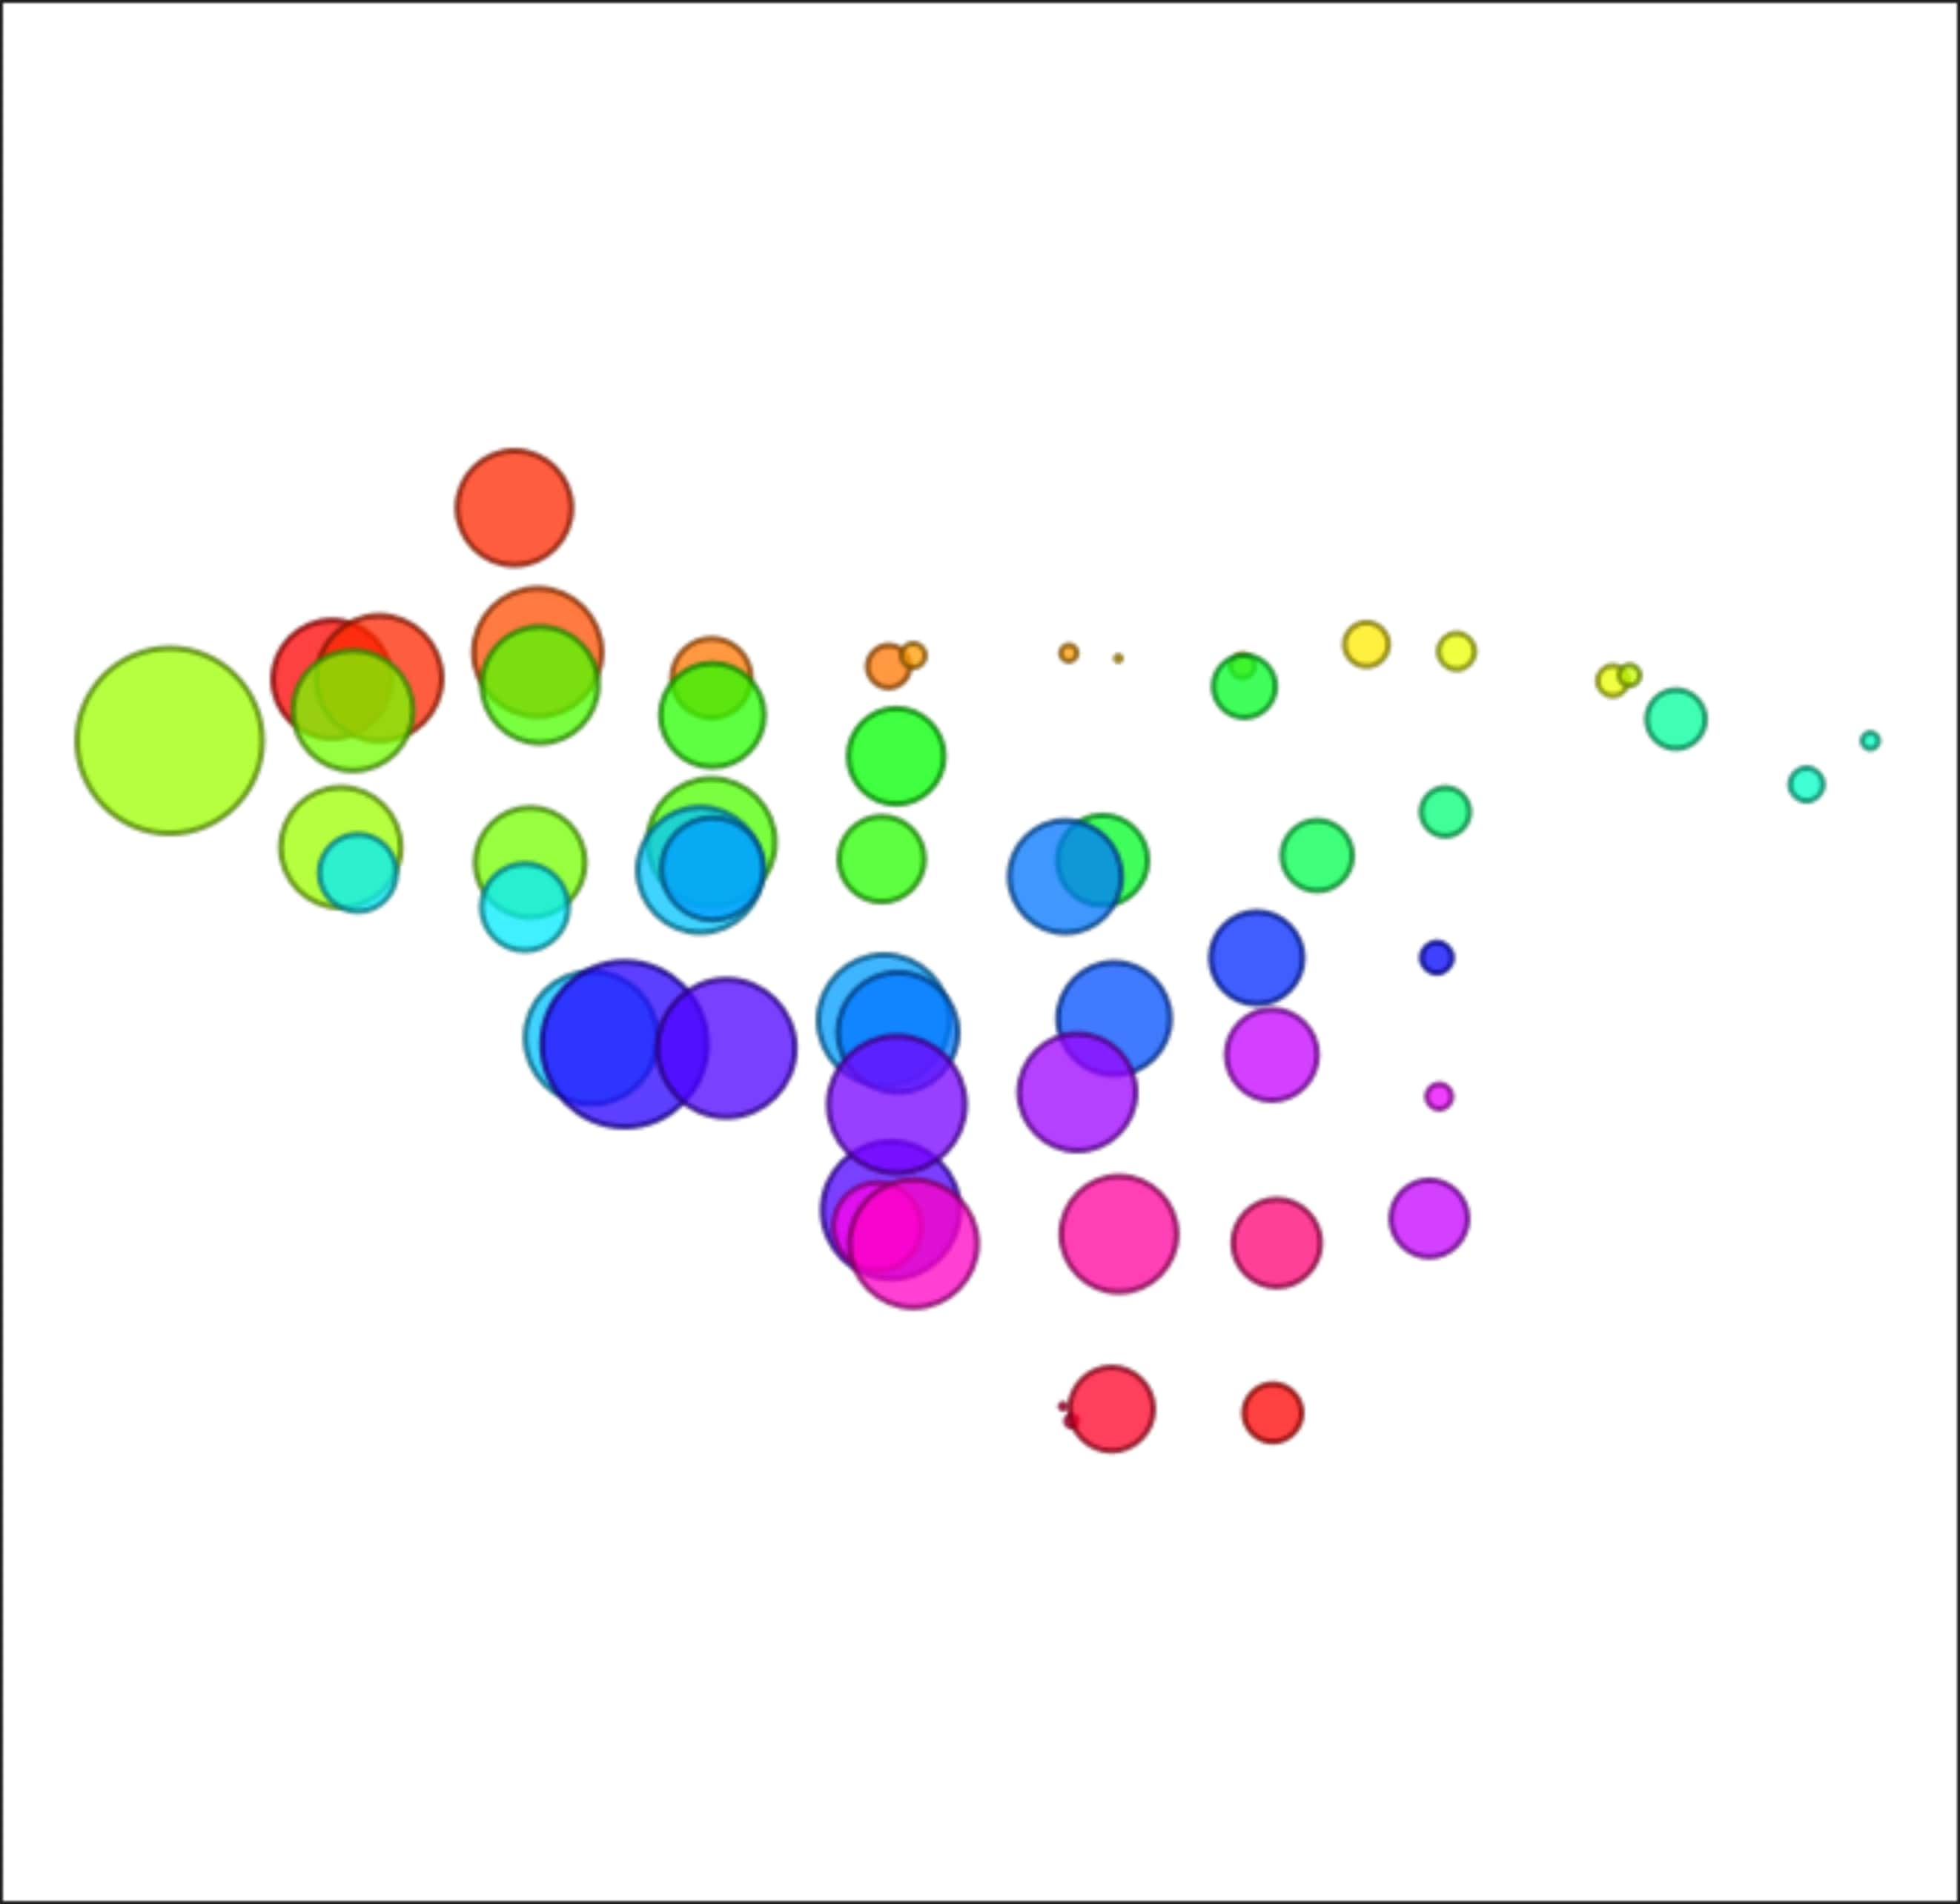
\includegraphics[width=0.6\columnwidth]{figs/tf-design-interface-a.jpg}}
    \hfill
    \subfloat[Fine-tune material classification after user adjustment.\label{subfig:tf-design-example-user}]{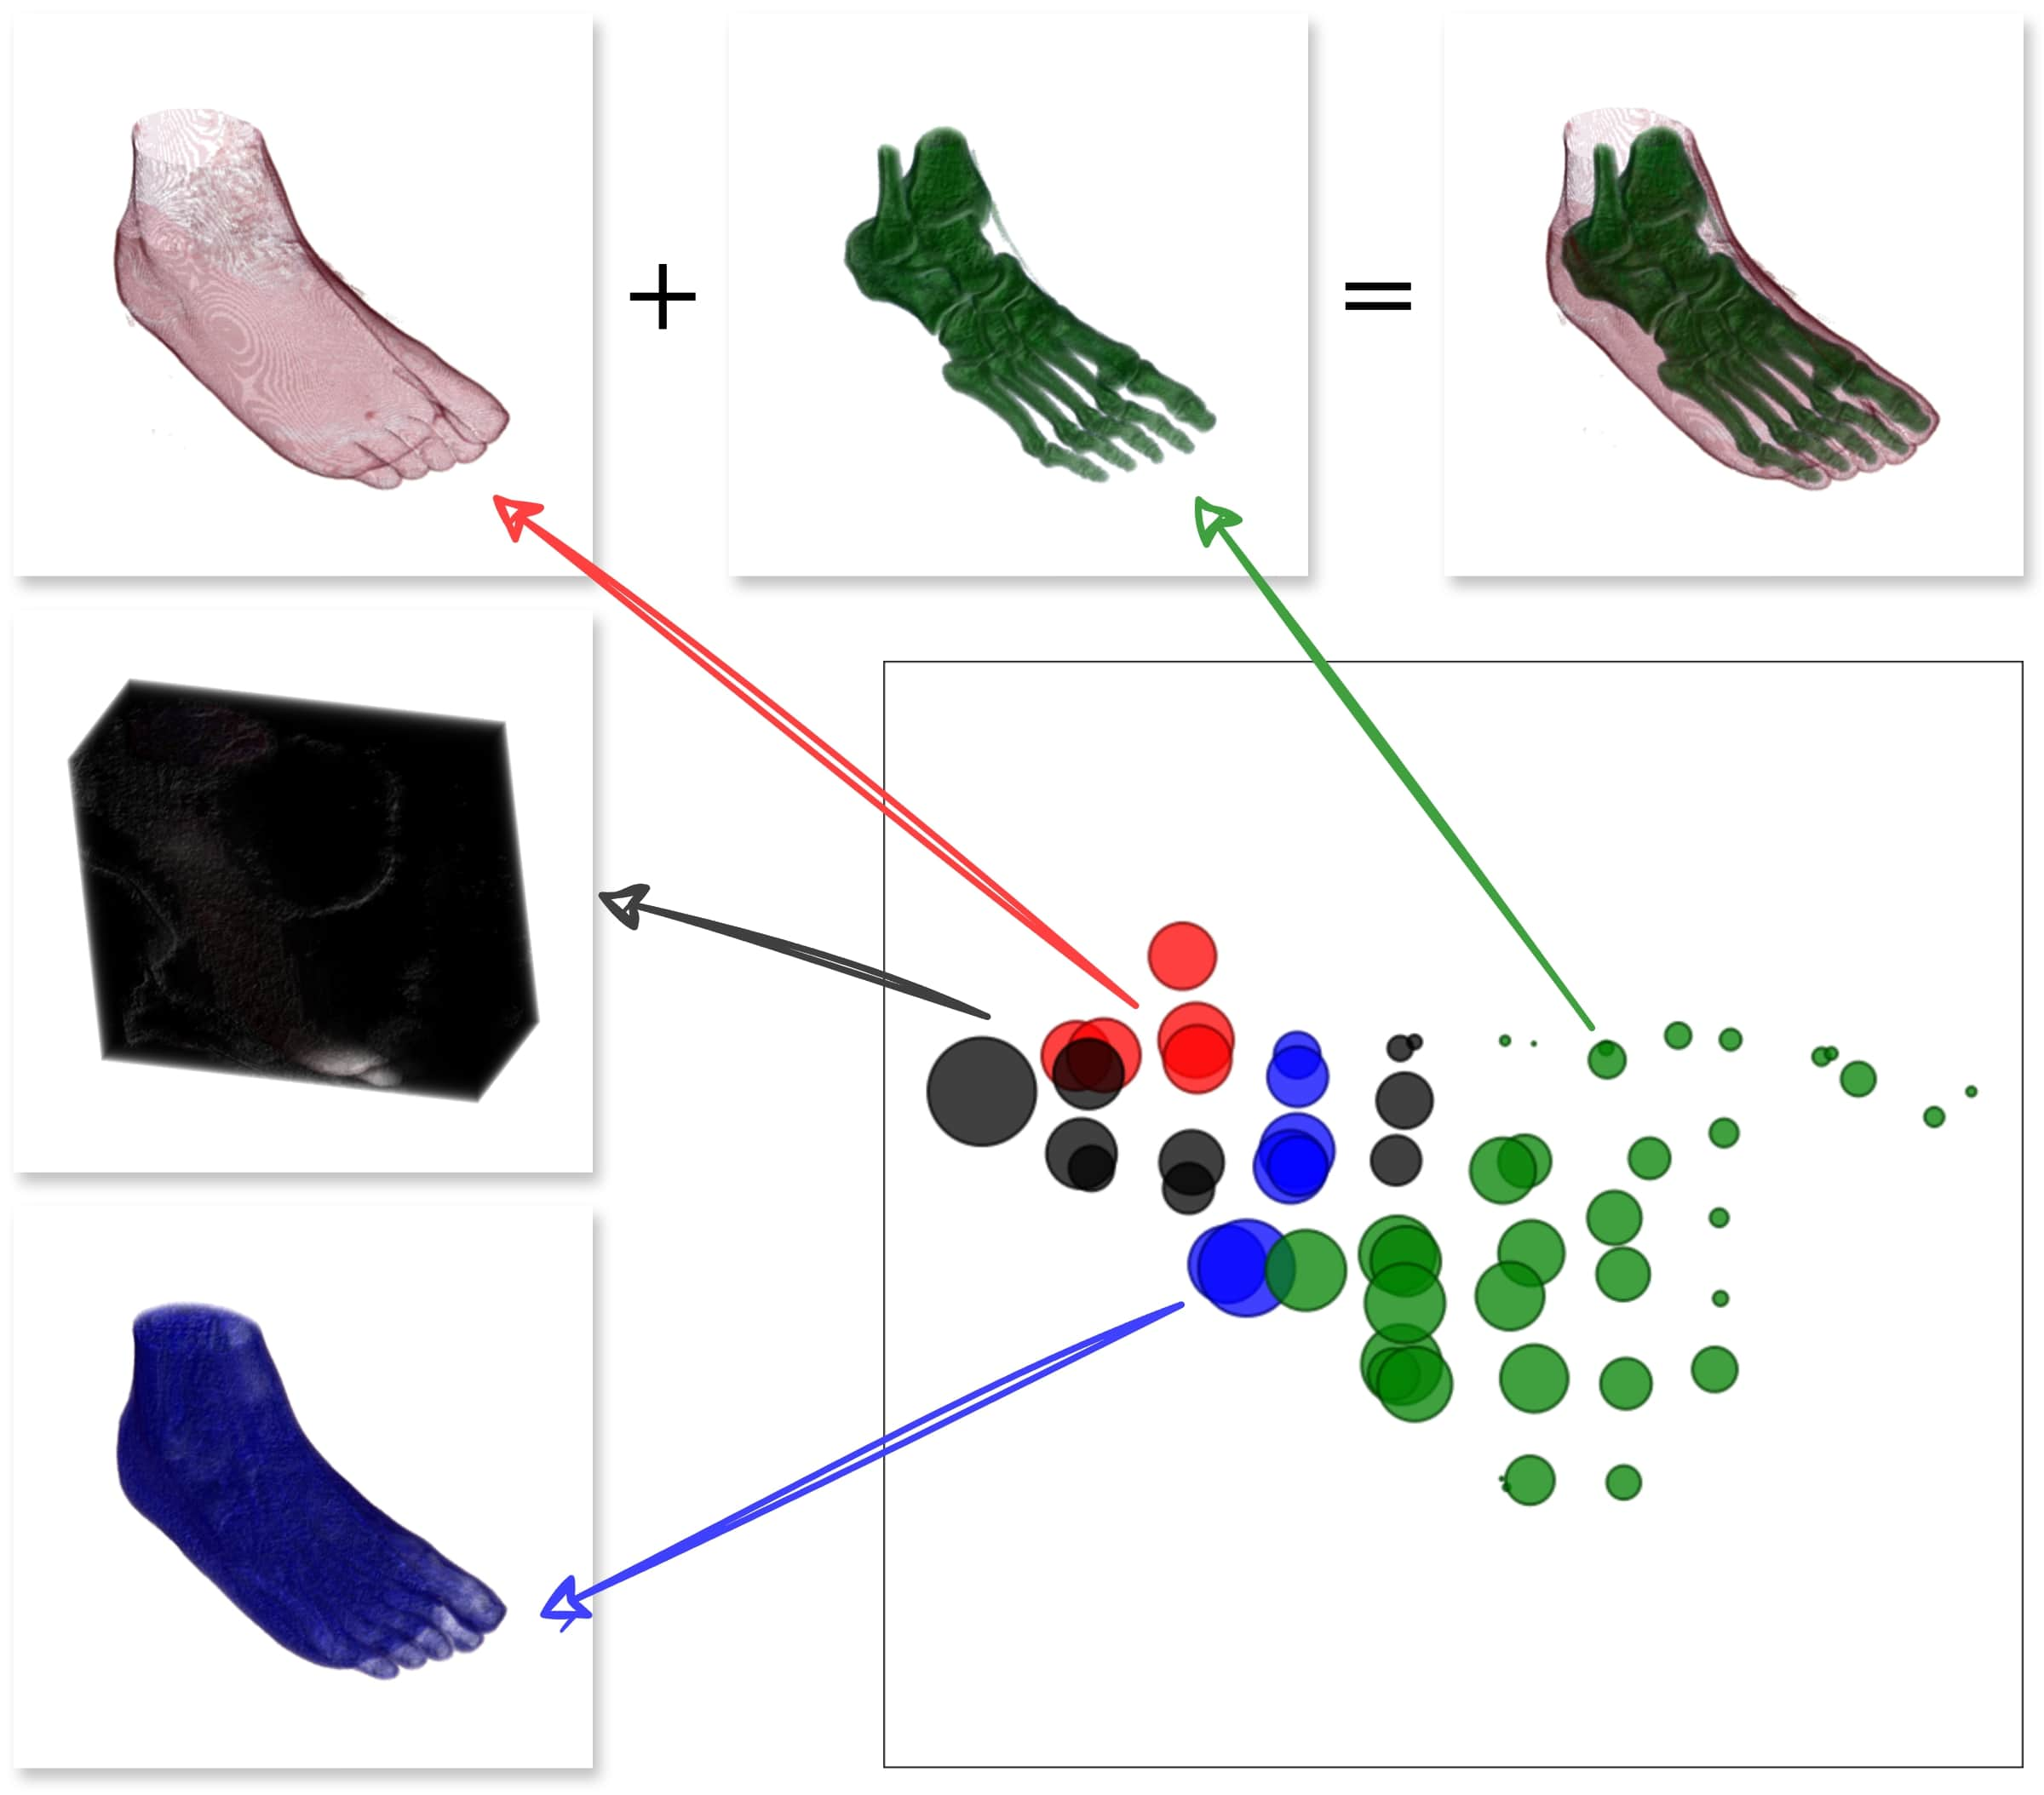
\includegraphics[width=0.6\columnwidth]{figs/tf-design-interface-b.jpg}}
    \caption{Transfer function design interface and volume exploration space of a right male foot dataset.}
    \label{fig:tf-design-example}
\end{figure}

Our method generates an initial TF specification using a predefined opacity and a rainbow color scale, assigning a unique color per cluster.

Users adjust the TF following the WYSIWYG principle: pivot color and opacity map directly to their associated voxels according to clustering. Both selected and unselected elements can be customized.

Volume exploration occurs through pivot selection. The system dynamically increases the opacity of selected pivots and decreases that of others. Users can make arbitrary selections, save them as groups, and interact with pivots, clusters, or groups as selectable entities.

Iterative selection of nearby elements aids identifying volume details. FastMap and DBSCAN naturally cluster similar instances spatially, simplifying this process.

Our approach automates material classification by assuming each cluster or pivot represents a relevant item. If unsatisfied, users may select/deselect elements or adjust parameters:

\begin{itemize}
    \item input volume data,
    \item DBSCAN parameters $\varepsilon$ and $minPts$,
    \item SSS distance factor $\alpha$.
\end{itemize}

\section{Results}
\label{sect:results}
\subsection{Experimental Design}
\label{subsect:experimental-design}

We conducted all the experiments on a computer equipped with an Intel Core I5 7200U, 8 GB RAM, running Ubuntu 22.04 64-bit, and an NVIDIA GeForce GT 940MX GPU. 

For image rendering, we utilized a classical volume-ray casting algorithm with Blinn-Phong illumination and trilinear interpolation. The ray step is adjusted according to voxel spacing. Our runtime analysis reflects the average of five trials. 

The system is implemented in C++, utilizing the Qt Framework and CUDA C/C++ for parallel processing. The implementation is available in online repositories.
%The system is implemented\footnotemark in C++, utilizing the Qt Framework and CUDA C/C++ for parallel processing. The implementation is available in online repositories.
% \footnotetext{An implementation is available  in \url{https://github.com/rafaelssantos/volumeexplorer}.}

Table~\ref{tab:datasets-descriptions} presents the datasets utilized in our experiments. These datasets are widely recognized within the volume visualization community and are publicly available through online repositories. The volume data consisted solely of material density, represented as intensity scalar values. The derived attributes are then used to generate multidimensional input. We consider 13 attributes, namely intensity, gradient magnitude, Laplacian magnitude, and 10 statistical measures computed from a local histogram. The statistical measures include absolute deviation, contrast, energy, entropy, inertia, Kurtosis, mean, skewness, standard deviation, and variance.

%Table~\ref{tab:datasets-descriptions} presents the datasets utilized in our experiments. These datasets are widely recognized within the volume visualization community and are publicly available through online repositories\footnotemark. The volume data consisted solely of material density, represented as intensity scalar values. The derived attributes are then used to generate multidimensional input. We consider 13 features, namely intensity, gradient magnitude, Laplacian magnitude, and 10 statistical measures computed from a local histogram. These statistical measures include absolute deviation, contrast, energy, entropy, inertia, Kurtosis, mean, skewness, standard deviation, and variance.
% \footnotetext{Volume dataset repository is available on \url{https://github.com/rafaelssantos/volume-datasets}.}

\begin{table}[htb!]
    \centering
    \caption{Volume datasets.}
    \begin{tabular}{@{}ccc@{}}
        \toprule
        \textbf{Dataset} & \textbf{Grid size} & \textbf{Total of voxels} \\ 
        \midrule
        Engine block & $256 \times 256 \times 256$ & 16,777,216\\
        Knees & $379 \times 229 \times 305$ & 26,471,255\\
        Tooth & $256 \times 256 \times 161$ & 10,551,296\\
        \bottomrule
        \label{tab:datasets-descriptions}
    \end{tabular}
\end{table}

The experiments generate rankings of attributes based on least squares regression error, MICI and correlation coefficient measures.

\subsection{Runtime}
\label{subsect:runtime-analysis}


Table~\ref{tab:runtime-analysis} presents the runtimes for the proposed method applied to each dataset.


\begin{table}[!htbp]
\caption{Runtime (in seconds) of the proposed method applied to each volume dataset.}
\label{tab:runtime-analysis}
\centering
    \begin{tabular}{@{}>{\centering\arraybackslash}m{0.4\columnwidth}>{\centering\arraybackslash}m{0.15\columnwidth}>{\centering\arraybackslash}m{0.15\columnwidth}>{\centering\arraybackslash}m{0.15\columnwidth}@{}}
        \toprule
            & \textbf{Block engine} & \textbf{Knees} & \textbf{Tooth}\\
        \midrule
        \textit{\textbf{Rankings of attributes}} & \textit{1540.50} & \textit{2430.00} & \textit{963.00} \\
        \hline
        \textbf{Feature extraction} & 7.50 & 7.98 & 36.05 \\
        \textbf{Clustering} & 51.52 & 102.77 & 19.42 \\
        \textbf{Pivot-based indexing} & 2.23 & 3.15 & 1.33 \\
        \midrule
        \textbf{Transfer function design interface} & 1.48 & 1.86 & 0.79 \\
        \bottomrule
    \end{tabular}
\end{table}

The feature selection process is not included in the runtime analysis, as it is performed manually. However, the calculation of attribute rankings is part of the analysis. It is pertinent to note that this step is computationally intensive compared to other method steps, with attribute rankings taking 15--40 minutes to generate. The remaining steps of the method took under two minutes for all tested datasets.

\subsection{Data classification}
\label{subsect:material-classification}

We use the heuristic proposed in Section~\ref{subsect:feature-selection} to search for a suitable TF for each dataset. Since the same number of attributes is available, we consistently began the investigation with $k = 4$, considering $d=13$ (where $k\approx \sqrt{13})$ available attributes. 

The DBSCAN parameter $minPts$ is default set~\cite{ester1996} as $4$ in all experiments. With the data normalized, we vary $\varepsilon$ between $\left[ 0.2, 0.35\right]$ and SSS parameter $\alpha$  between $\left[0.8, 0.95\right]$ to simulate volume exploration.

\subsubsection{Engine block dataset}
\label{subsubsec:engine-block}

Fig.~\ref{fig:engine-block-clusters-tf} shows the volume exploration space generated for the engine block dataset. Each numbered group is a classified volume detail rendered as presented in Fig.~\ref{fig:engine-block-clusters}. The method parameters are set as follows: $k=4$, TF $=\{$intensity, skewness, gradient magnitude and variance$\}$; $minPts = 4$; $\varepsilon = 0.35$; and $\alpha = 0.85$. 

\begin{figure}[htb!]
    \centering
    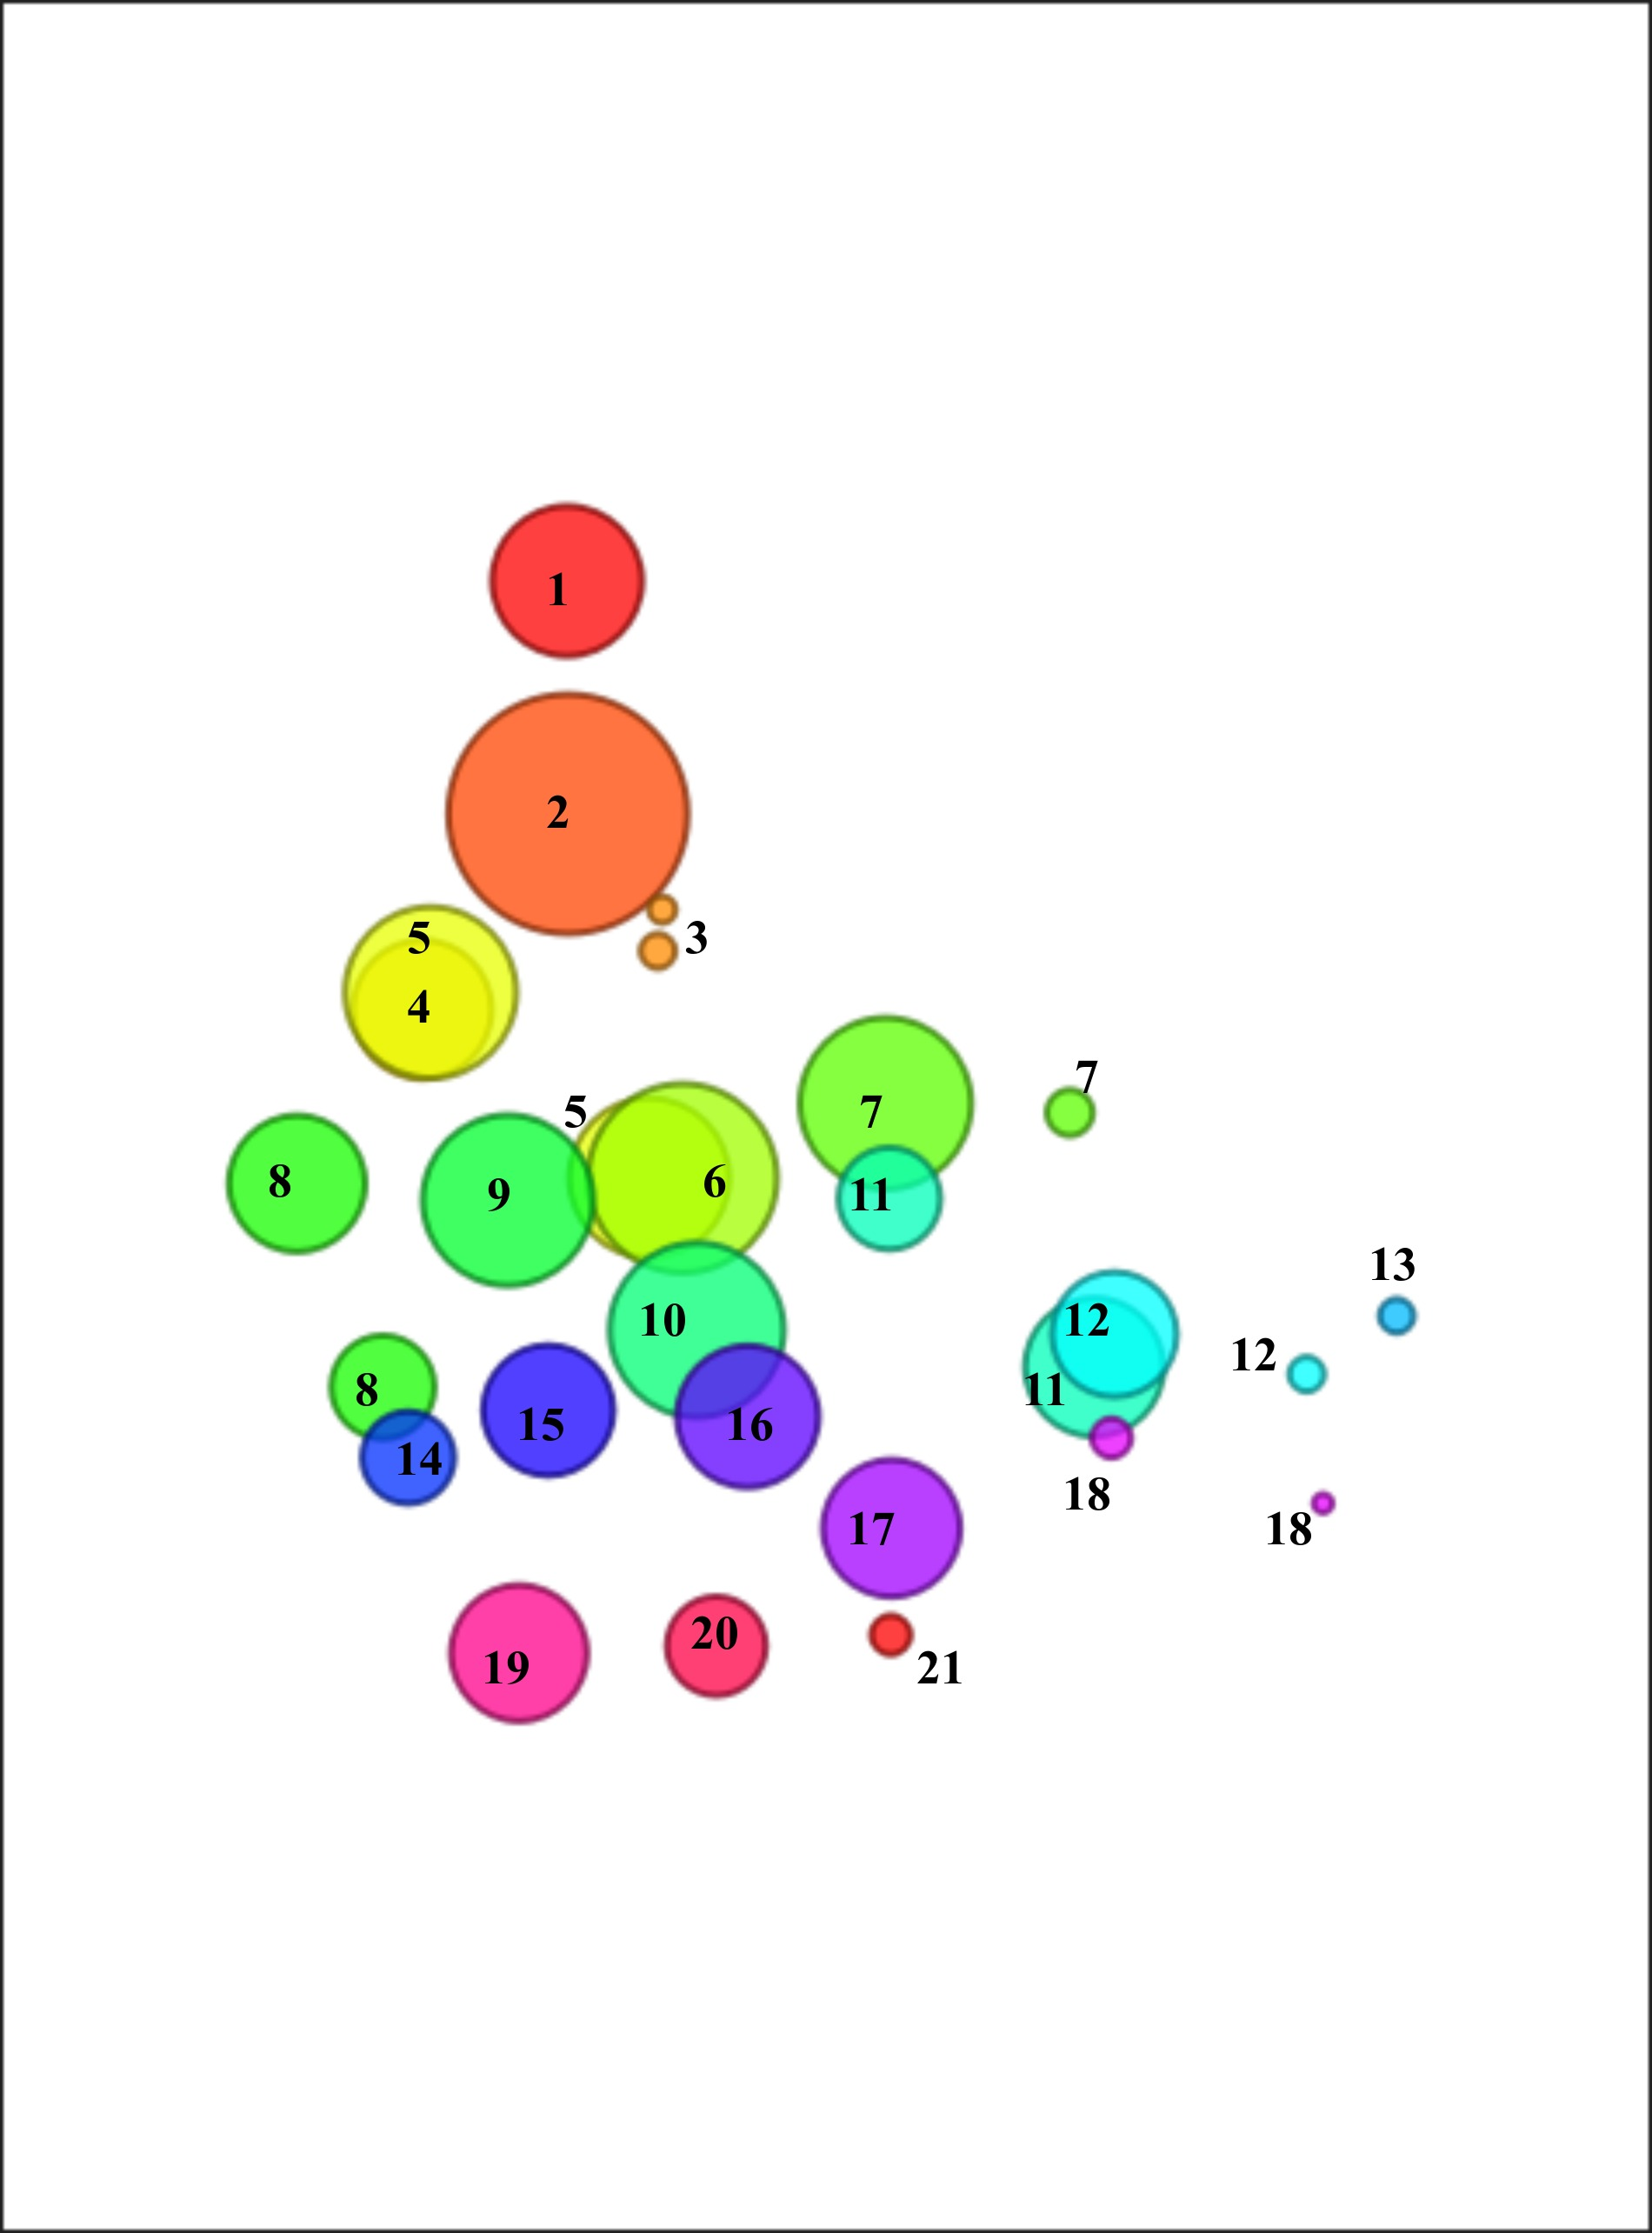
\includegraphics[width=0.7\columnwidth]{figs/engine-block-clusters-tf.jpg}
    \caption{Volume exploration space for the engine block dataset. Method parameters setup: transfer function $=\{$intensity, skewness, gradient magnitude and variance$\}$; $minPts = 4$;  $\varepsilon = 0.35$; and $\alpha = 0.85$.}
    \label{fig:engine-block-clusters-tf}
\end{figure}

\begin{figure}[htb!]
    \centering
    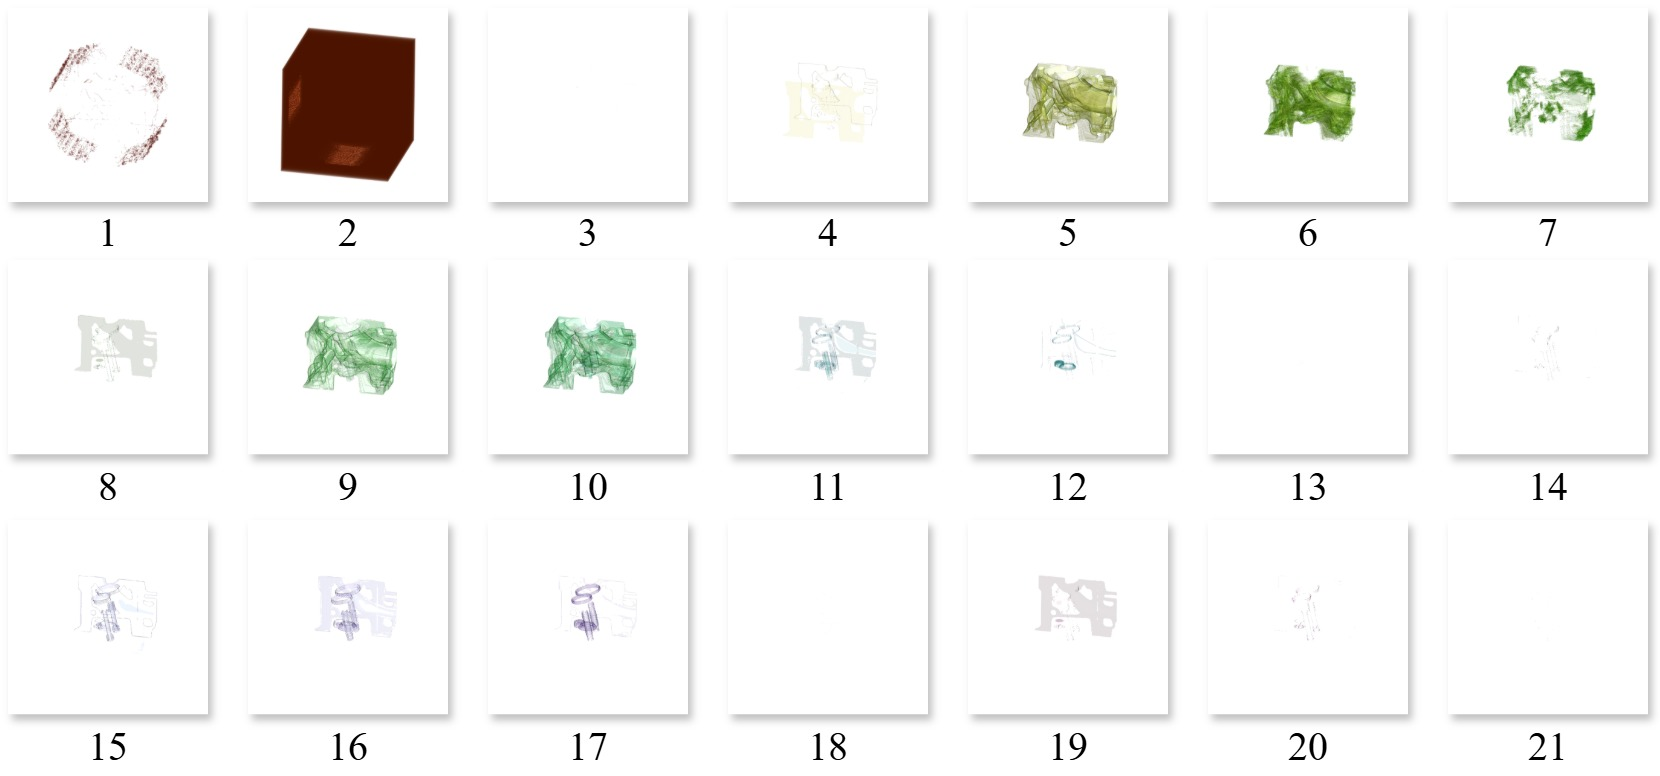
\includegraphics[width=\columnwidth]{figs/engine-block-clusters.jpg}
    \caption{Rendered volume classification details for the engine block dataset. Method parameters setup: transfer function  $=\{$intensity, skewness, gradient magnitude and variance$\}$; $minPts = 4$; $\varepsilon = 0.35$; and $\alpha = 0.85$.}
    \label{fig:engine-block-clusters}
\end{figure}

The rankings of attributes for the engine block dataset are shown in Table~\ref{tab:feature-ranking-for-engine-block}. We obtained the best results with the one based on the correlation coefficient measure.

\begin{table}[htb!]
    \caption{Rankings of volume data attributes for the engine block dataset.}
    \label{tab:feature-ranking-for-engine-block}
    \centering
    \begin{tabular}{@{}c>{\centering\arraybackslash}m{0.27\columnwidth}>{\centering\arraybackslash}m{0.27\columnwidth}>{\centering\arraybackslash}m{0.27\columnwidth}@{}}
        \toprule
         \textbf{$\#$} & \textbf{Least Squares Regression Error} & \textbf{Maximal Information Compression Index} & \textbf{Correlation Coefficient}\\
        \midrule
        $1$ & Intensity &  Intensity &  Intensity \\
        \hline
        $2$ & Energy &  Variance &  Skewness \\
        \hline
        $3$ & Inertia &  Absolute deviation & Gradient Magnitude \\
        \hline
        $4$ & Entropy &  Energy &  Variance \\
        \hline
        $5$ & Skewness &  Contrast &  Laplacian Magnitude \\
        \hline
        $6$ & Mean &  Entropy &  Entropy \\
        \hline
        $7$ & Absolute deviation &  Gradient Magnitude &  Energy \\
        \hline
        $8$ & Laplacian Magnitude &  Inertia &  Inertia \\
        \hline
        $9$ & Kurtosis &  Kurtosis &  Standard deviation \\
        \hline
        $10$ & Standard deviation &  Laplacian Magnitude &  Mean \\
        \hline
        $11$ & Gradient Magnitude &  Mean &  Kurtosis \\
        \hline
        $12$ & Contrast &  Skewness &  Absolute deviation \\
        \hline
        $13$ & Variance &  Standard deviation &  Contrast \\
        \bottomrule
    \end{tabular}
\end{table}

A volume exploration simulation is demonstrated in Fig.~\ref{fig:engine-block-groups}. It reveals different engine block components. The process happens from the initial setup presented in Fig.~\ref{fig:engine-block-clusters-tf}. 

\begin{figure}[htb!]
    \centering
    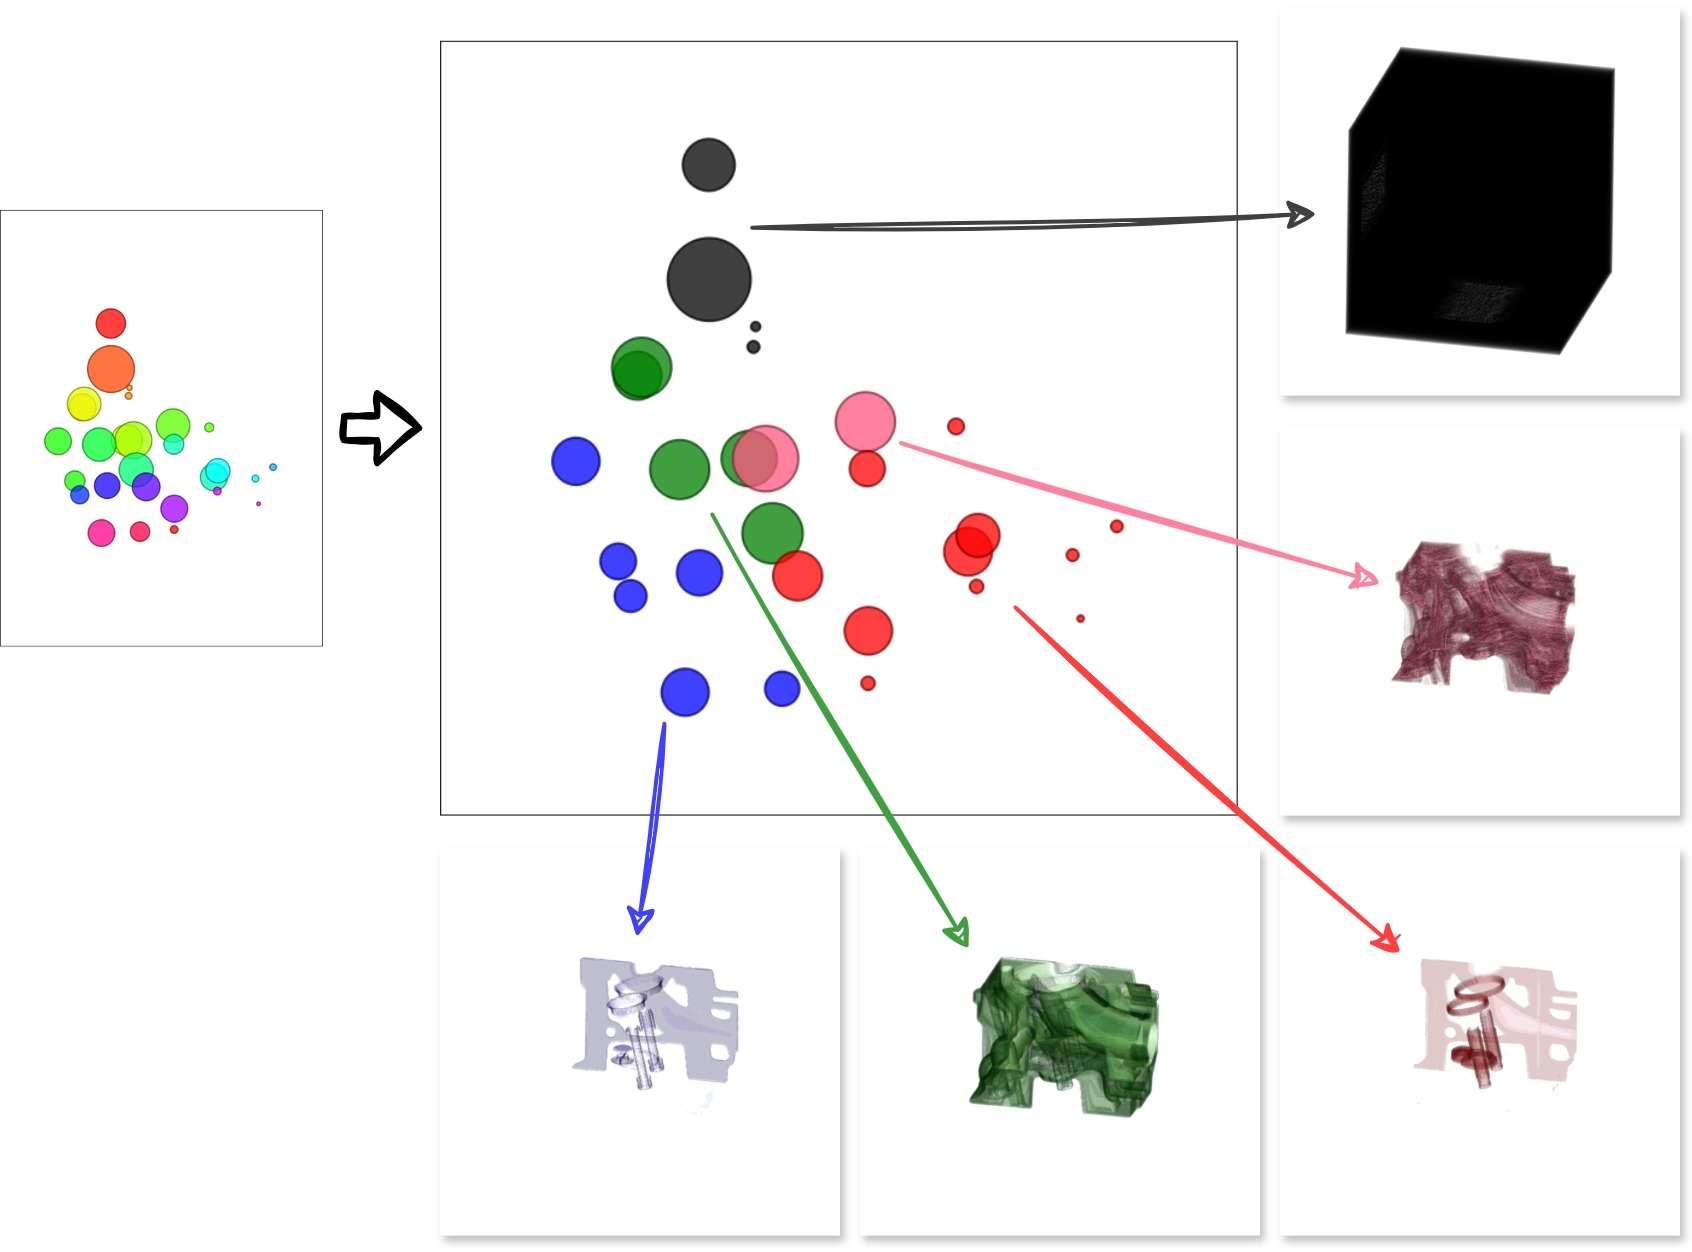
\includegraphics[width=\columnwidth]{figs/engine-block-groups.jpg}
    \caption{Visual analysis of user-refined transfer function design and volume classification for engine block datasets. The volume details are manually grouped from an empirical perspective. Method parameters setup: transfer function $=\{$intensity, skewness, gradient magnitude and variance$\}$; $minPts = 4$; $\varepsilon = 0.35$; and $\alpha = 0.85$.}
    \label{fig:engine-block-groups}
\end{figure}



\subsubsection{Knees dataset}
\label{subsubsect:knees-dataset}
A preliminary volume classification for knees datasets is presented in Fig.~\ref{fig:knees-tf-clusters} and the related rendered details in Fig.~\ref{fig:knees-clusters}. The method parameters are set as follows:  TF $=\{$intensity,  variance, absolute deviation, energy and contrast$\}$; $minPts = 4$; $\varepsilon = 0.35$; and $\alpha = 0.9$. 


\begin{figure}[htb!]
    \centering
    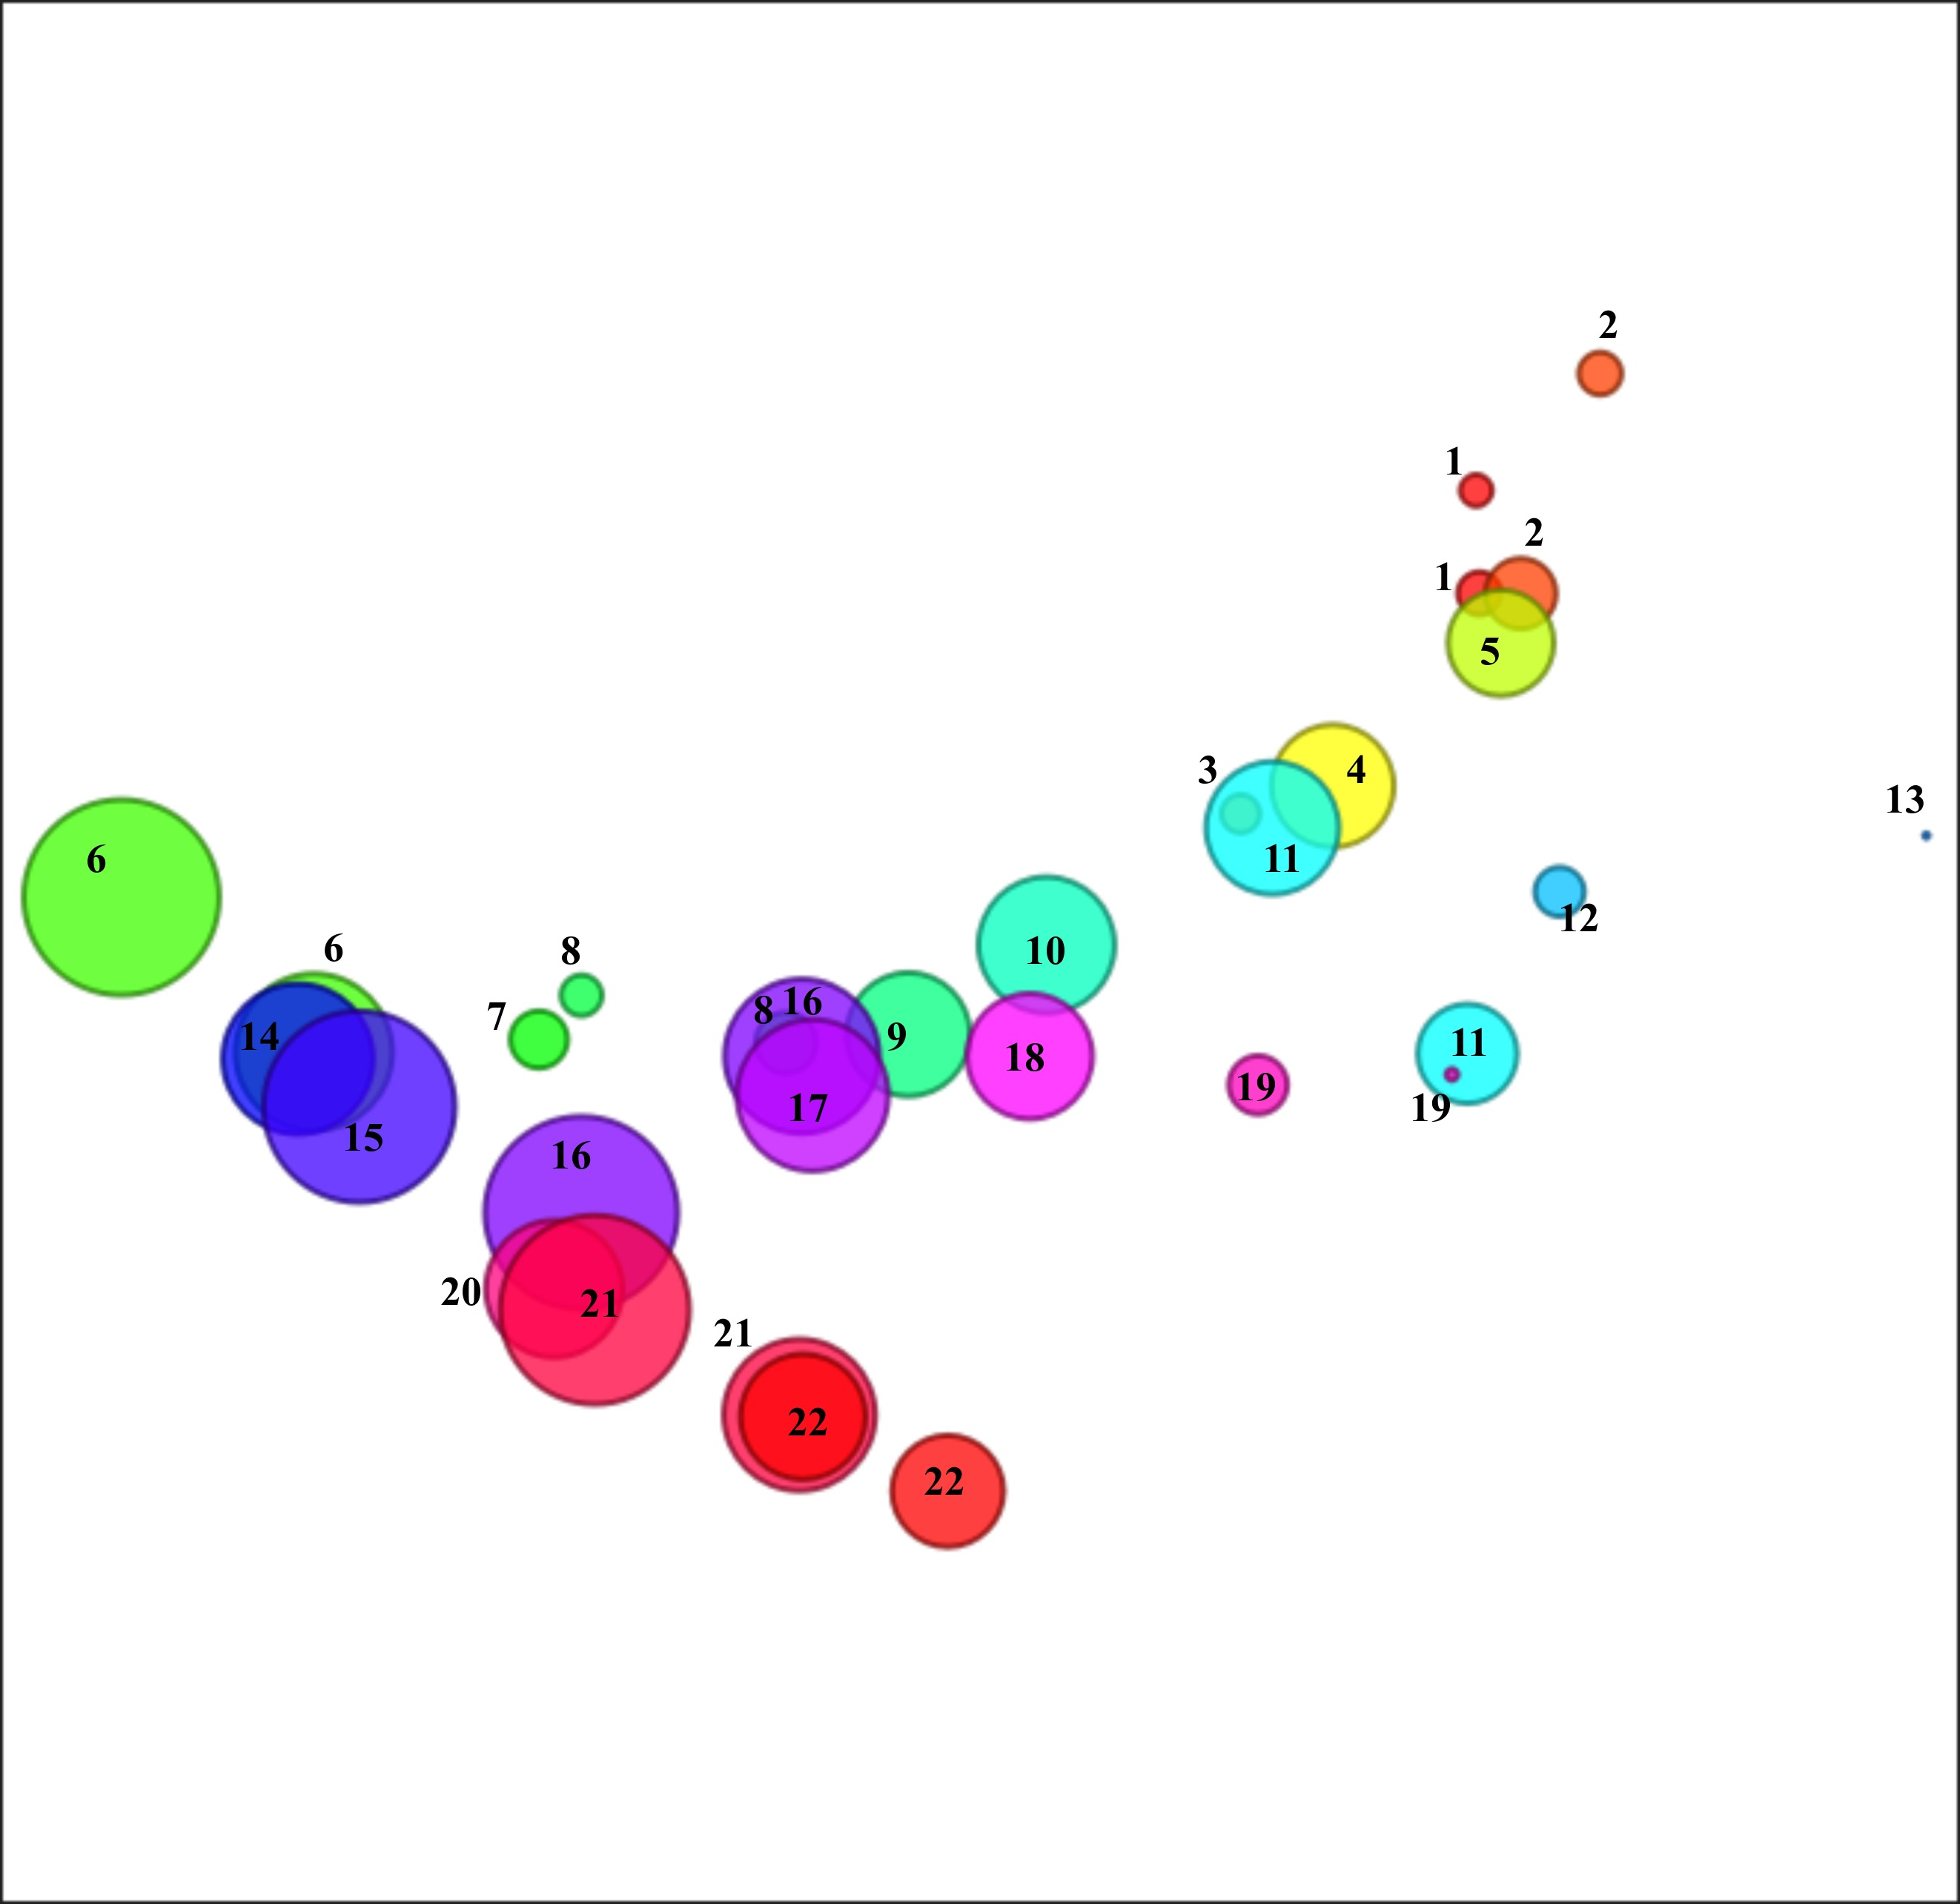
\includegraphics[width=0.7\columnwidth]{figs/knees-clusters-tf.jpg} 
     \caption{Volume exploration space for the knees dataset. Method parameters setup: transfer function $=\{$intensity,  variance, absolute deviation, energy and contrast$\}$; $minPts = 4$; $\varepsilon = 0.35$; and $\alpha = 0.9$.}
    \label{fig:knees-tf-clusters}
\end{figure}

\begin{figure}[htb!]
    \centering
    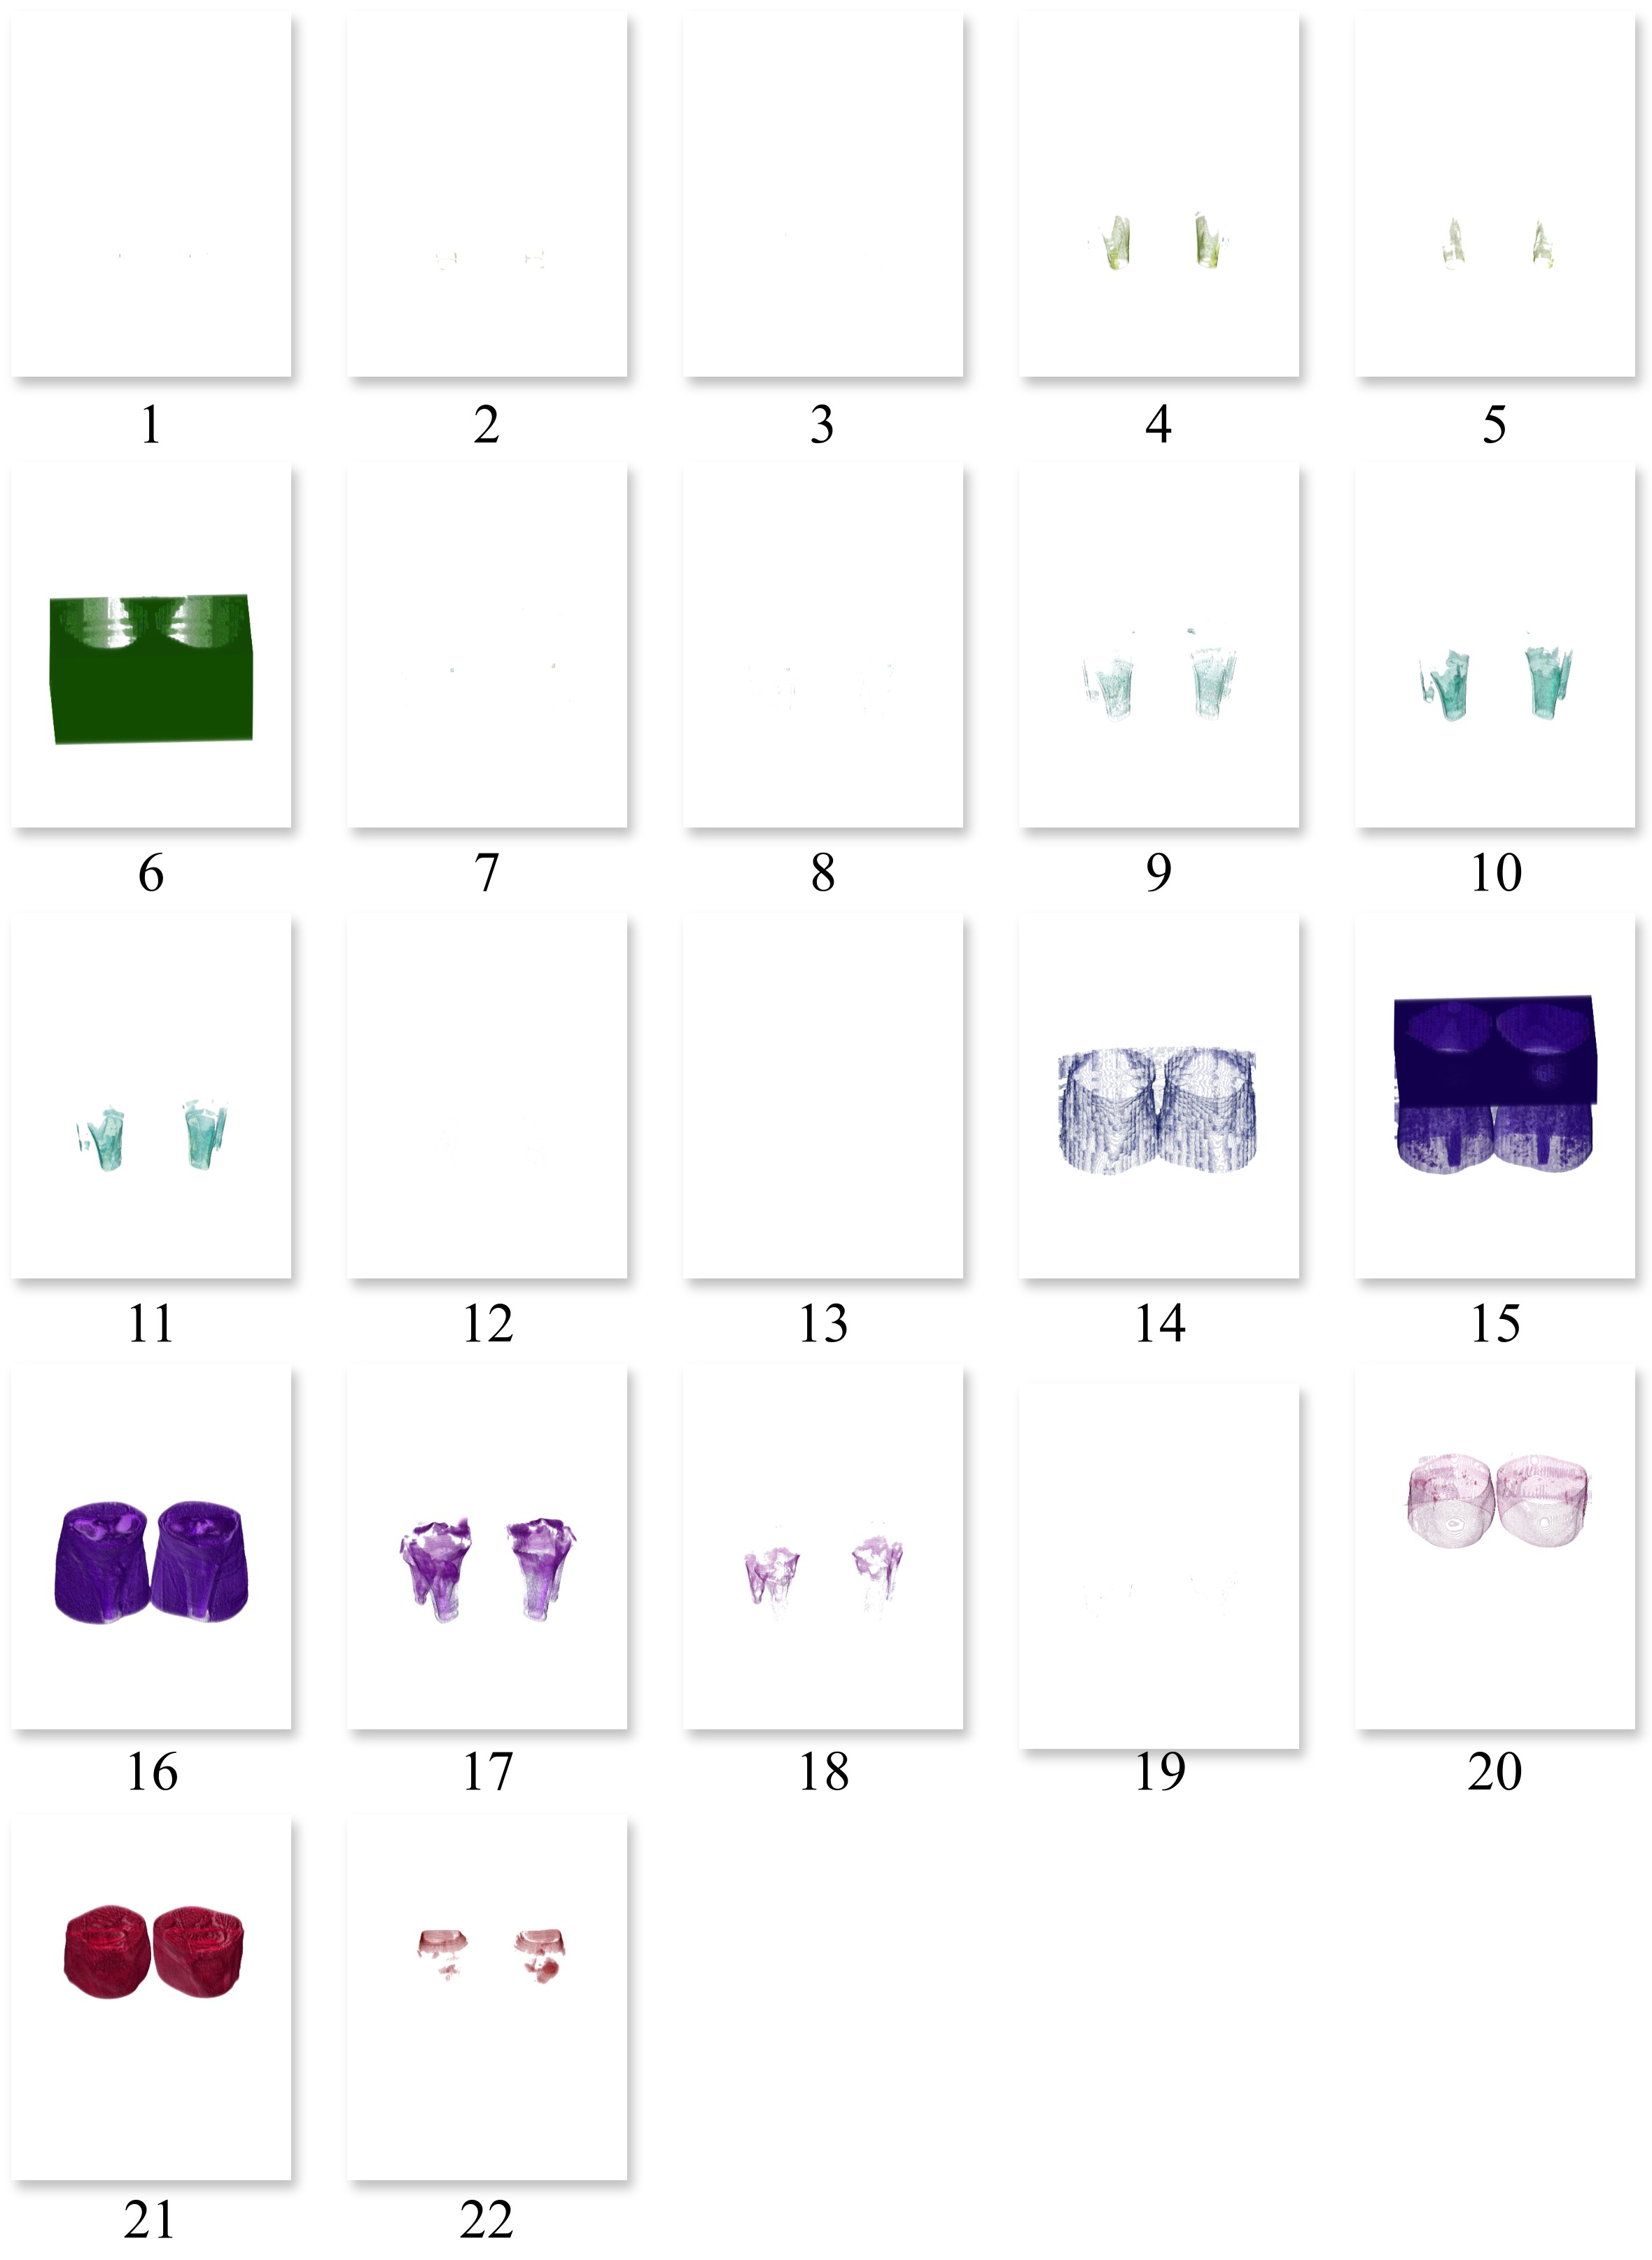
\includegraphics[width=\columnwidth]{figs/knees-clusters.jpg} 
     \caption{Rendered volume classification details for the knees dataset. Method parameters setup: transfer function $=\{$intensity,  variance, absolute deviation, energy and contrast$\}$; $minPts = 4$; $\varepsilon = 0.35$; and $\alpha = 0.9$.}
    \label{fig:knees-clusters}
\end{figure}

Table~\ref{tab:feature-ranking-for-tooth} presents the rankings generated for the tooth dataset.  We use the MICI measure ranking for the TF definition.

\begin{table}[htb!]
    \caption{Rankings of volume data attributes for the knees dataset.}
    \label{tab:feature-ranking-for-knees}
    \centering
    \begin{tabular}{@{}c>{\centering\arraybackslash}m{0.27\columnwidth}>{\centering\arraybackslash}m{0.27\columnwidth}>{\centering\arraybackslash}m{0.27\columnwidth}@{}}
        \toprule
         \textbf{$\#$} & \textbf{Least Squares Regression Error} & \textbf{Maximal Information Compression Index} & \textbf{Correlation Coefficient}\\
        \midrule
        $1$ & Intensity &  Intensity &  Intensity \\
        \hline
        $2$ & Entropy &  Variance &  Variance \\
        \hline
        $3$ & Energy &  Absolute deviation &  Skewness \\
        \hline
        $4$ & Inertia &  Energy &  Entropy \\
        \hline
        $5$ & Skewness &  Contrast &  Energy \\
        \hline
        $6$ & Laplacian Magnitude &  Entropy &  Inertia \\
        \hline
        $7$ & Mean &  Gradient Magnitude &  Standard deviation \\
        \hline
        $8$ & Absolute deviation &  Inertia &  Laplacian Magnitude \\
        \hline
        $9$ & Kurtosis &  Kurtosis &  Gradient Magnitude \\
        \hline
        $10$ & Standard deviation &  Laplacian Magnitude &  Kurtosis \\
        \hline
        $11$ & Gradient Magnitude &  Mean &  Absolute deviation \\
        \hline
        $12$ & Contrast &  Skewness &  Mean \\
        \hline
        $13$ & Variance &  Standard deviation &  Contrast \\
        \bottomrule
    \end{tabular}
\end{table}

By exploring the volume details, it is possible to group and identify bones and muscular structures. Fig.~\ref{fig:knees-groups} illustrates these structures, which include parts of the femur, tibia, patella, fibula, thigh muscles, and knee muscles.

\begin{figure}[htb!]
    \centering
    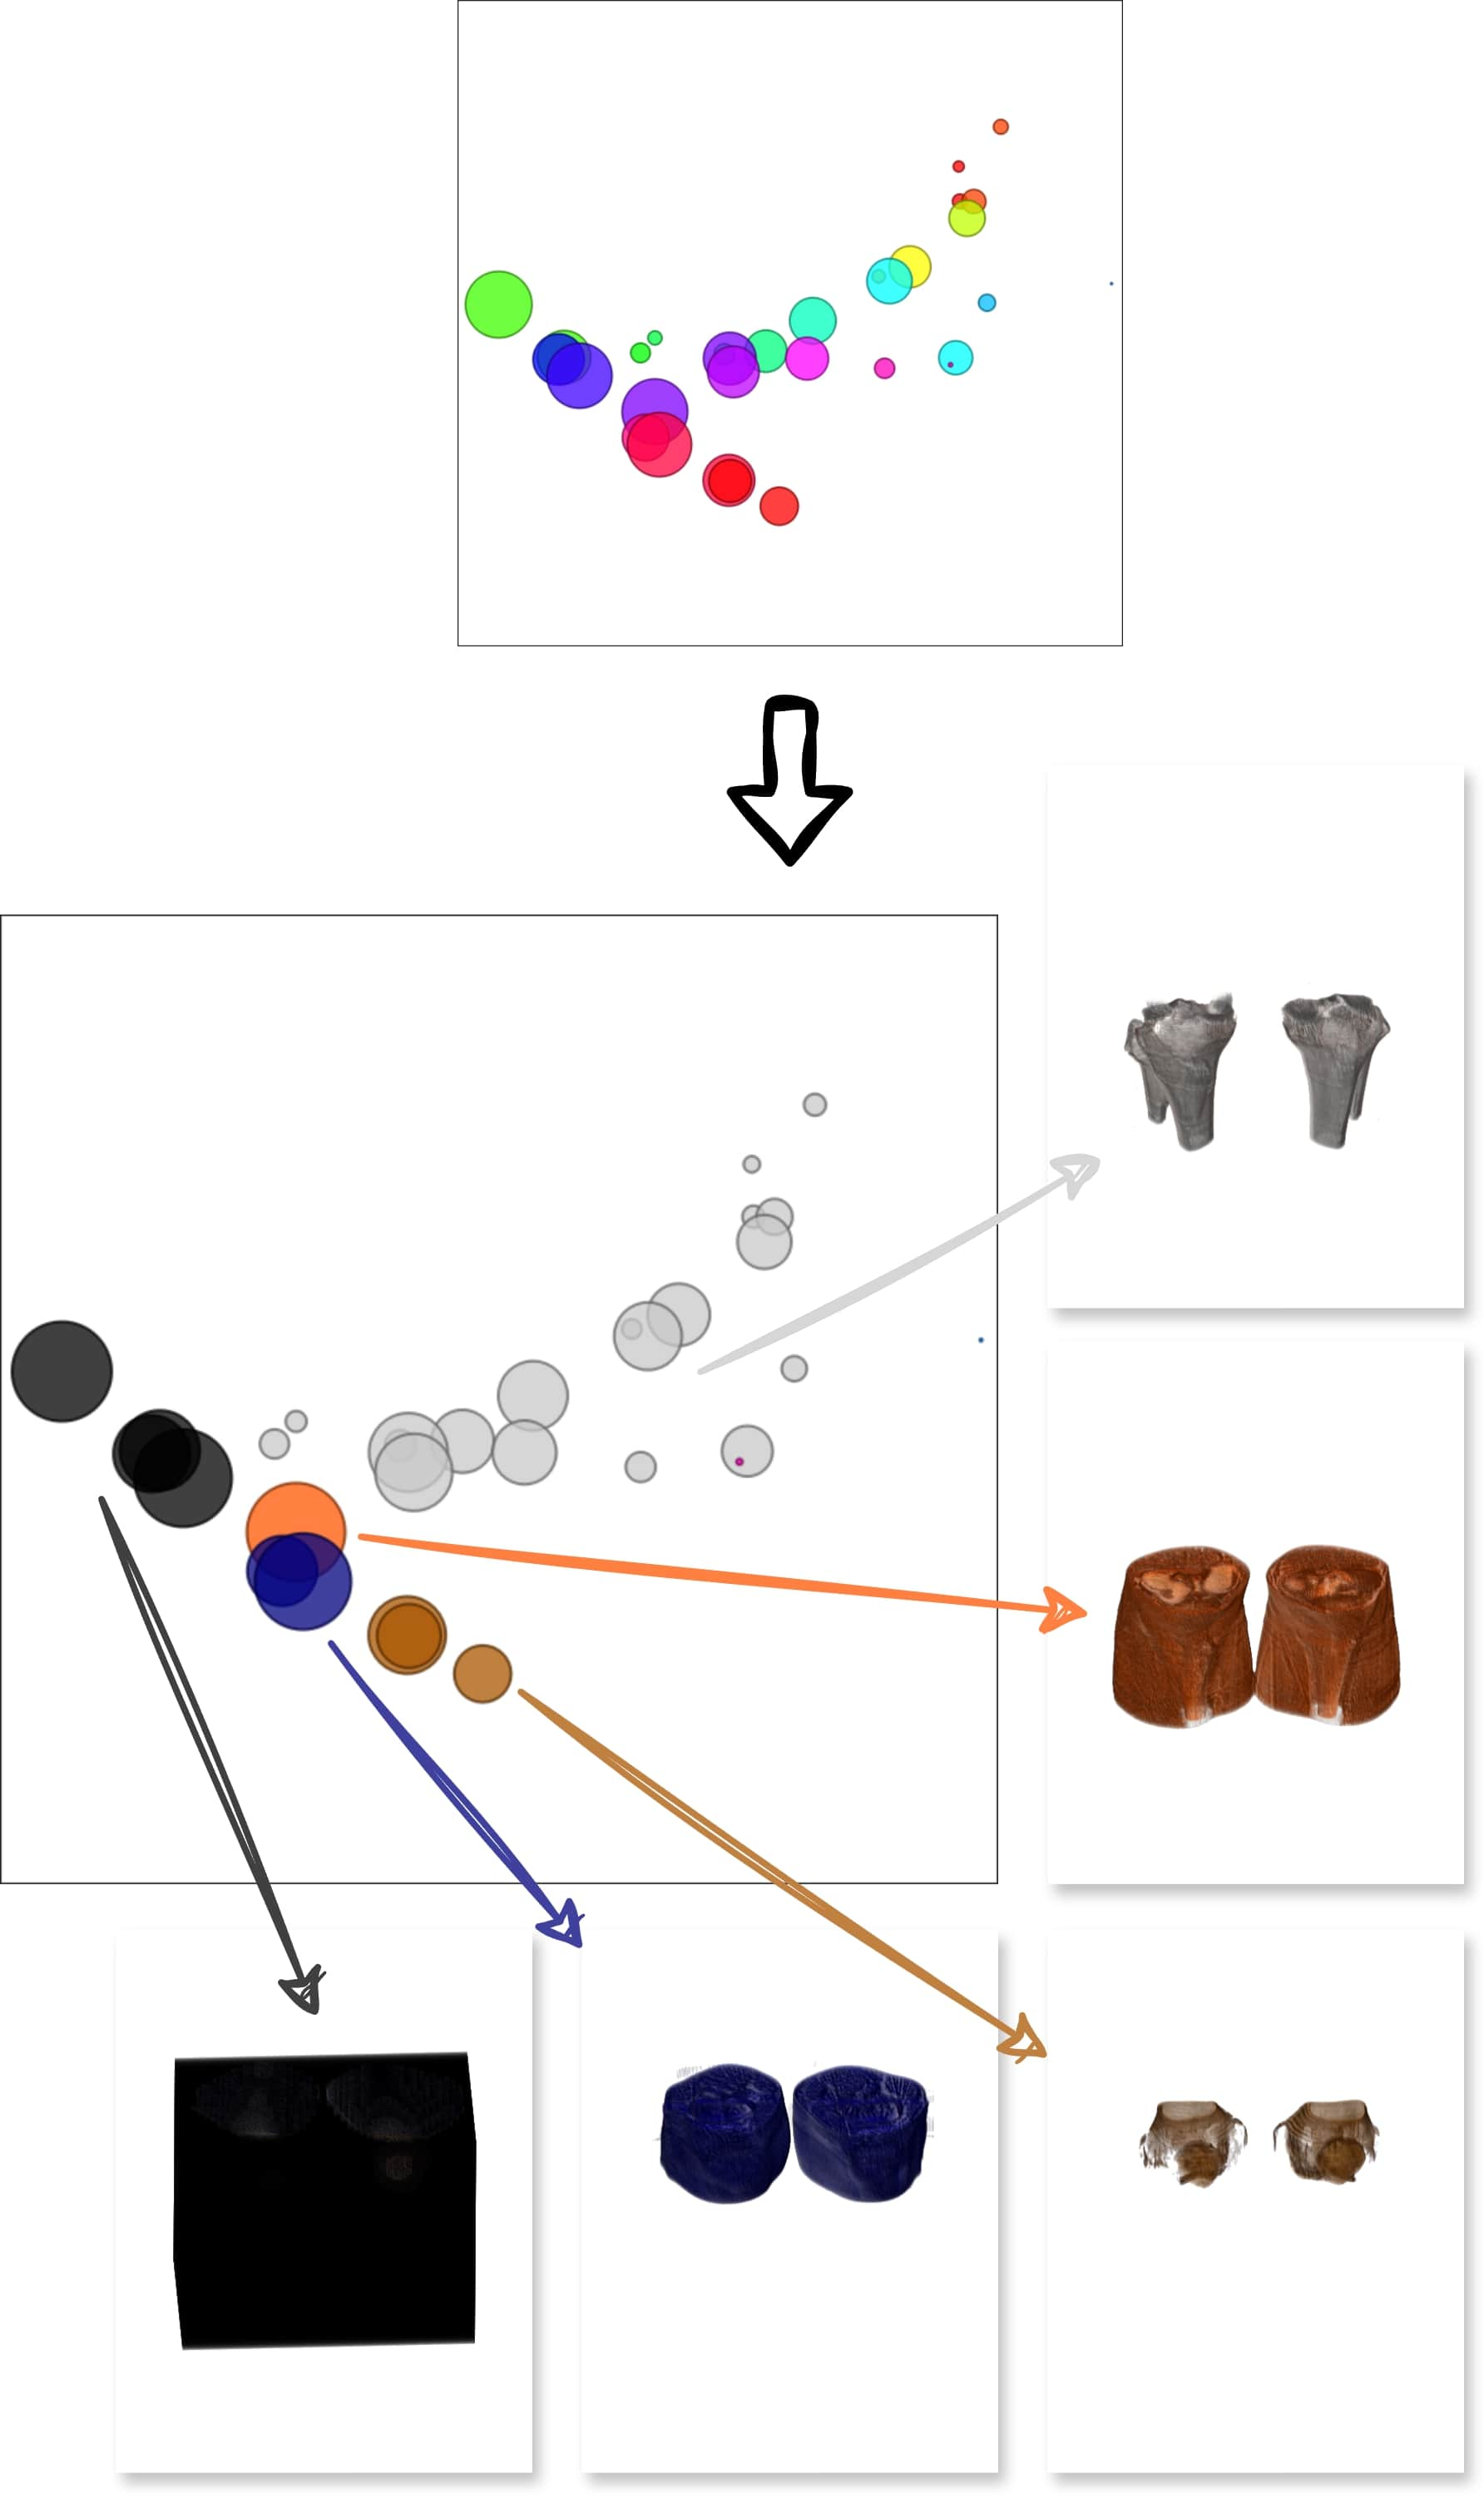
\includegraphics[width=\columnwidth]{figs/knees-groups.jpg}
    \caption{Visual analysis of user-refined transfer function design and volume classification for knees dataset. The volume details are manually grouped from an empirical perspective. Method parameters setup: transfer function $=\{$intensity,  variance, absolute deviation, energy and contrast$\}$; $minPts = 4$; $\varepsilon = 0.35$; and $\alpha = 0.9$.}
    \label{fig:knees-groups}
\end{figure}




\subsubsection{Tooth dataset}
\label{subsubsect:tooth-dataset}
Fig.~\ref{fig:tooth-clusters} presents  visualizations of a tooth dataset classification. The method parameters are set as follows:  TF $= \{$intensity, variance, absolute deviation, energy, contrast and entropy$\}$; $minPts = 4$; $\varepsilon = 0.23$; and $\alpha = 0.9$.

Table~\ref{tab:feature-ranking-for-tooth}  outlines the attribute dissimilarity rankings. The ranking based on the MICI measure is which one is chosen to support the TF definition. 

\begin{figure}[htb!]
    \centering
    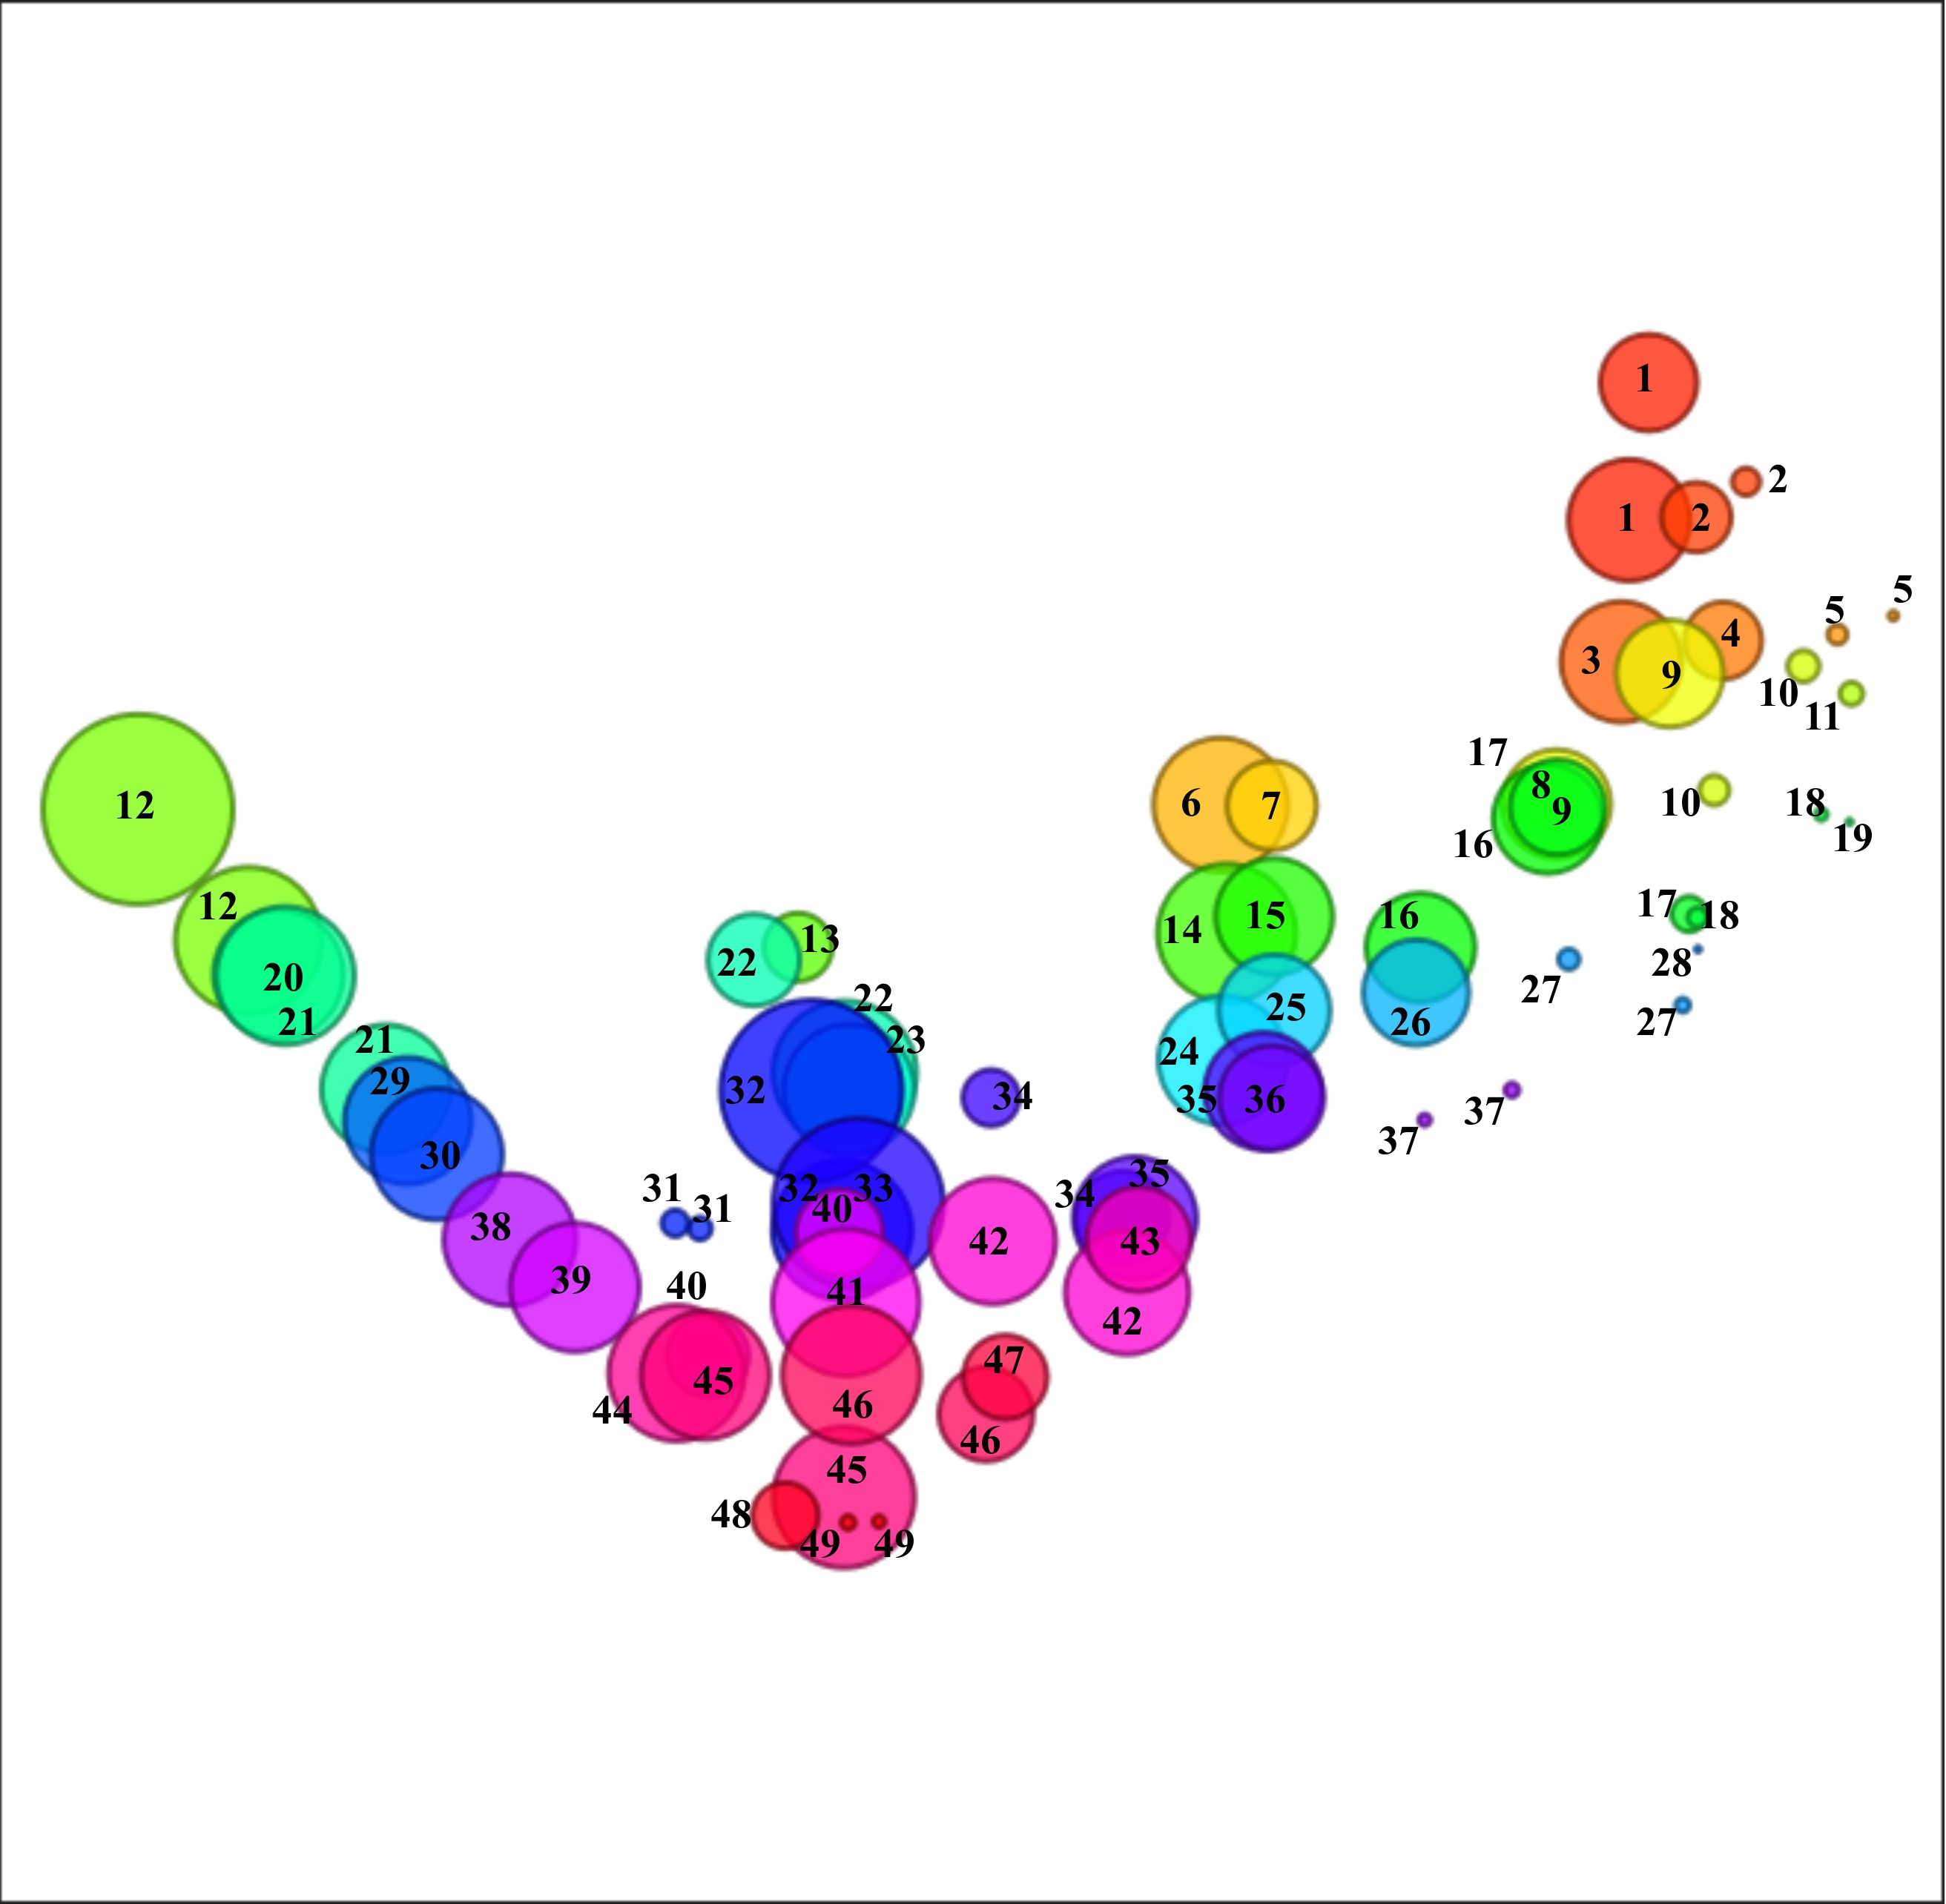
\includegraphics[width=0.7\columnwidth]{figs/tooth-clusters-tf.jpg} 
    \caption{Volume exploration space for the tooth dataset. Method parameters setup: transfer function $ =\{$intensity, variance, absolute deviation, energy, contrast and entropy$\}$; $minPts = 4$; $\varepsilon = 0.23$; and $\alpha = 0.9$.}
    \label{fig:tooth-clusters}
\end{figure}

\begin{figure}[htb!]
    \centering
    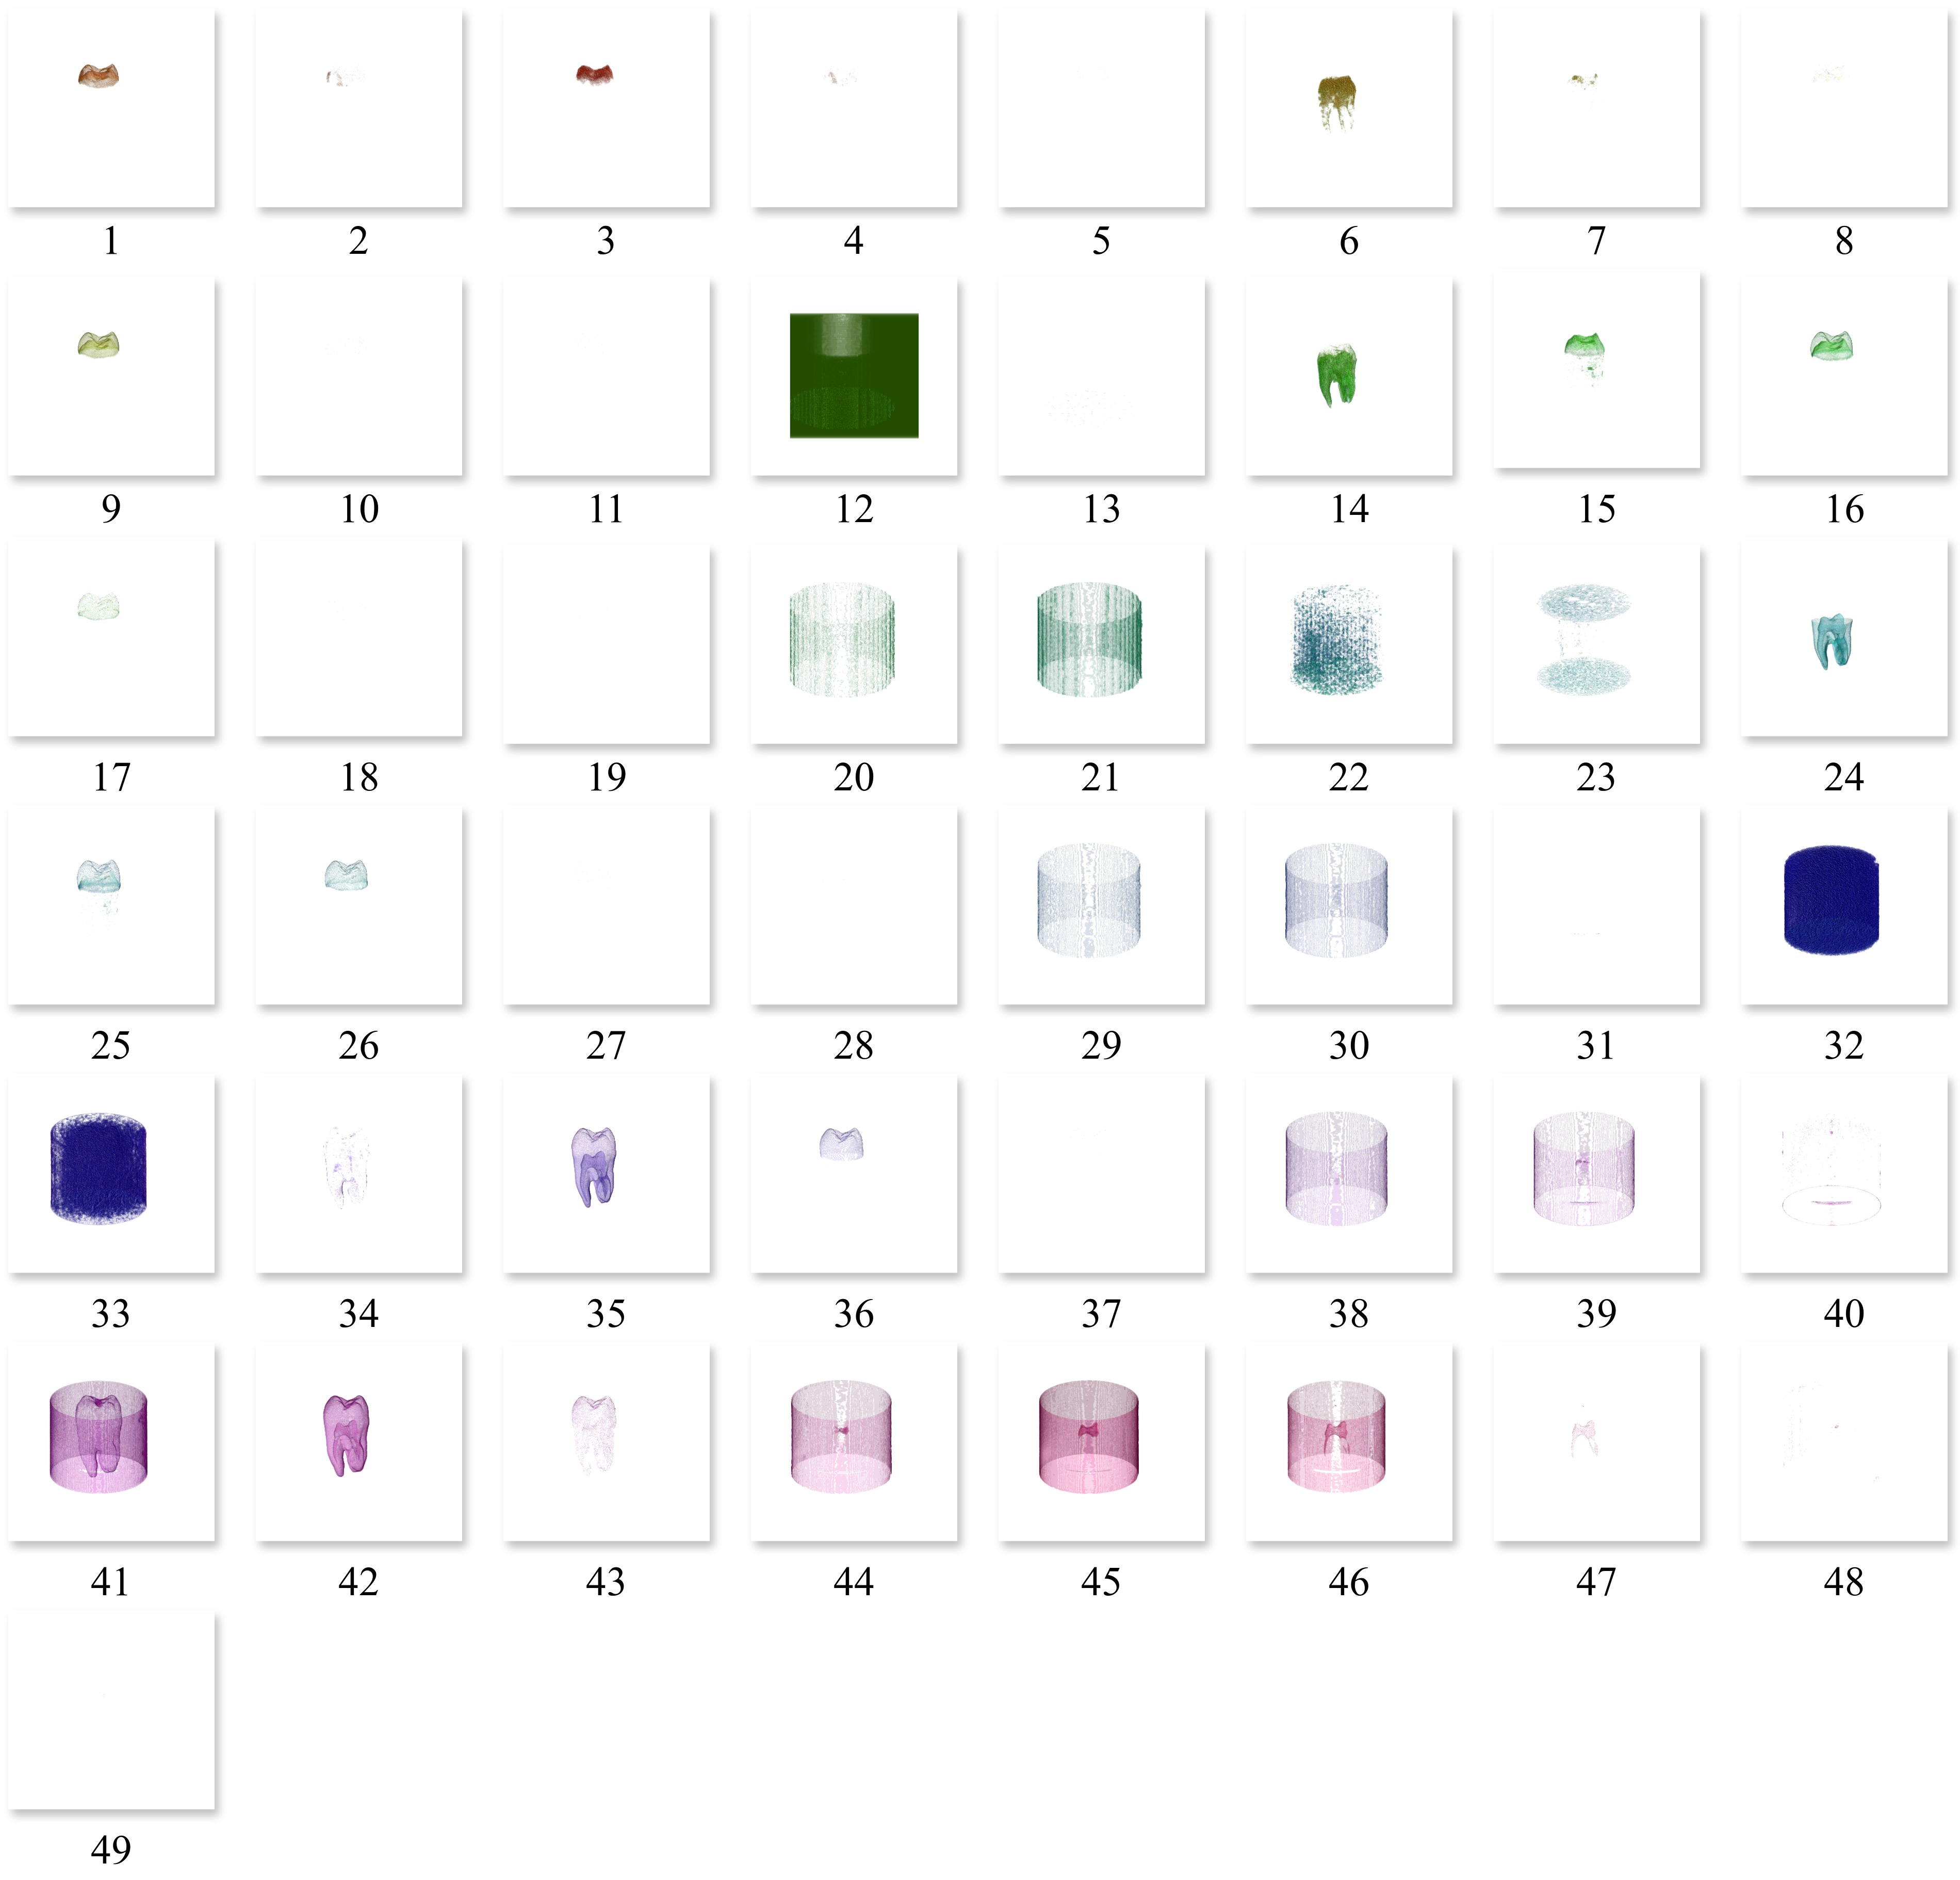
\includegraphics[width=\columnwidth]{figs/tooth-clusters.jpg} 
    \caption{Rendered volume classification details for the tooth dataset. The method parameters are set as follows: transfer function $ =\{$intensity, variance, absolute deviation, energy, contrast and entropy$\}$; $minPts = 4$; $\varepsilon = 0.23$; and $\alpha = 0.9$.}
    \label{fig:tooth-clusters}
\end{figure}


Manually generated groups of related tooth details are presented in Fig.~\ref{fig:tooth-groups}.  It shows several discernible structures, including the enamel, pulp, dentin, crown, the entire tooth, and the fluid in which it is immersed.

\begin{table}[htb!]
    \centering
    \caption{Rankings of volume data attributes for the tooth dataset.}
    \label{tab:feature-ranking-for-tooth}
    \begin{tabular}{@{}c>{\centering\arraybackslash}m{0.27\columnwidth}>{\centering\arraybackslash}m{0.27\columnwidth}>{\centering\arraybackslash}m{0.27\columnwidth}@{}}
        \toprule
         \textbf{$\#$} & \textbf{Least Square Regression Error} & \textbf{Maximal Information Compression Index} & \textbf{Correlation Coefficient}\\
        \midrule
        $1$ & Intensity &  Intensity &  Intensity \\
        \hline
        $2$ & Energy &  Variance &  Variance \\
        \hline
        $3$ & Inertia &  Absolute deviation &  Skewness \\
        \hline
        $4$ & Entropy &  Energy &  Gradient Magnitude \\
        \hline
        $5$ & Skewness &  Contrast &  Laplacian Magnitude \\
        \hline
        $6$ & Laplacian Magnitude &  Entropy &  Energy \\
        \hline
        $7$ & Mean &  Gradient Magnitude &  Inertia \\
        \hline
        $8$ & Absolute deviation &  Inertia &  Standard deviation \\
        \hline
        $9$ & Kurtosis &  Kurtosis &  Entropy \\
        \hline
        $10$ & Gradient Magnitude &  Laplacian Magnitude &  Kurtosis \\
        \hline
        $11$ & Standard deviation &  Mean &  Absolute deviation \\
        \hline
        $12$ & Contrast &  Skewness &  Mean \\
        \hline
        $13$ & Variance &  Standard deviation &  Contrast \\
        \bottomrule
    \end{tabular}
\end{table}

\begin{figure}[htb!]
    \centering
    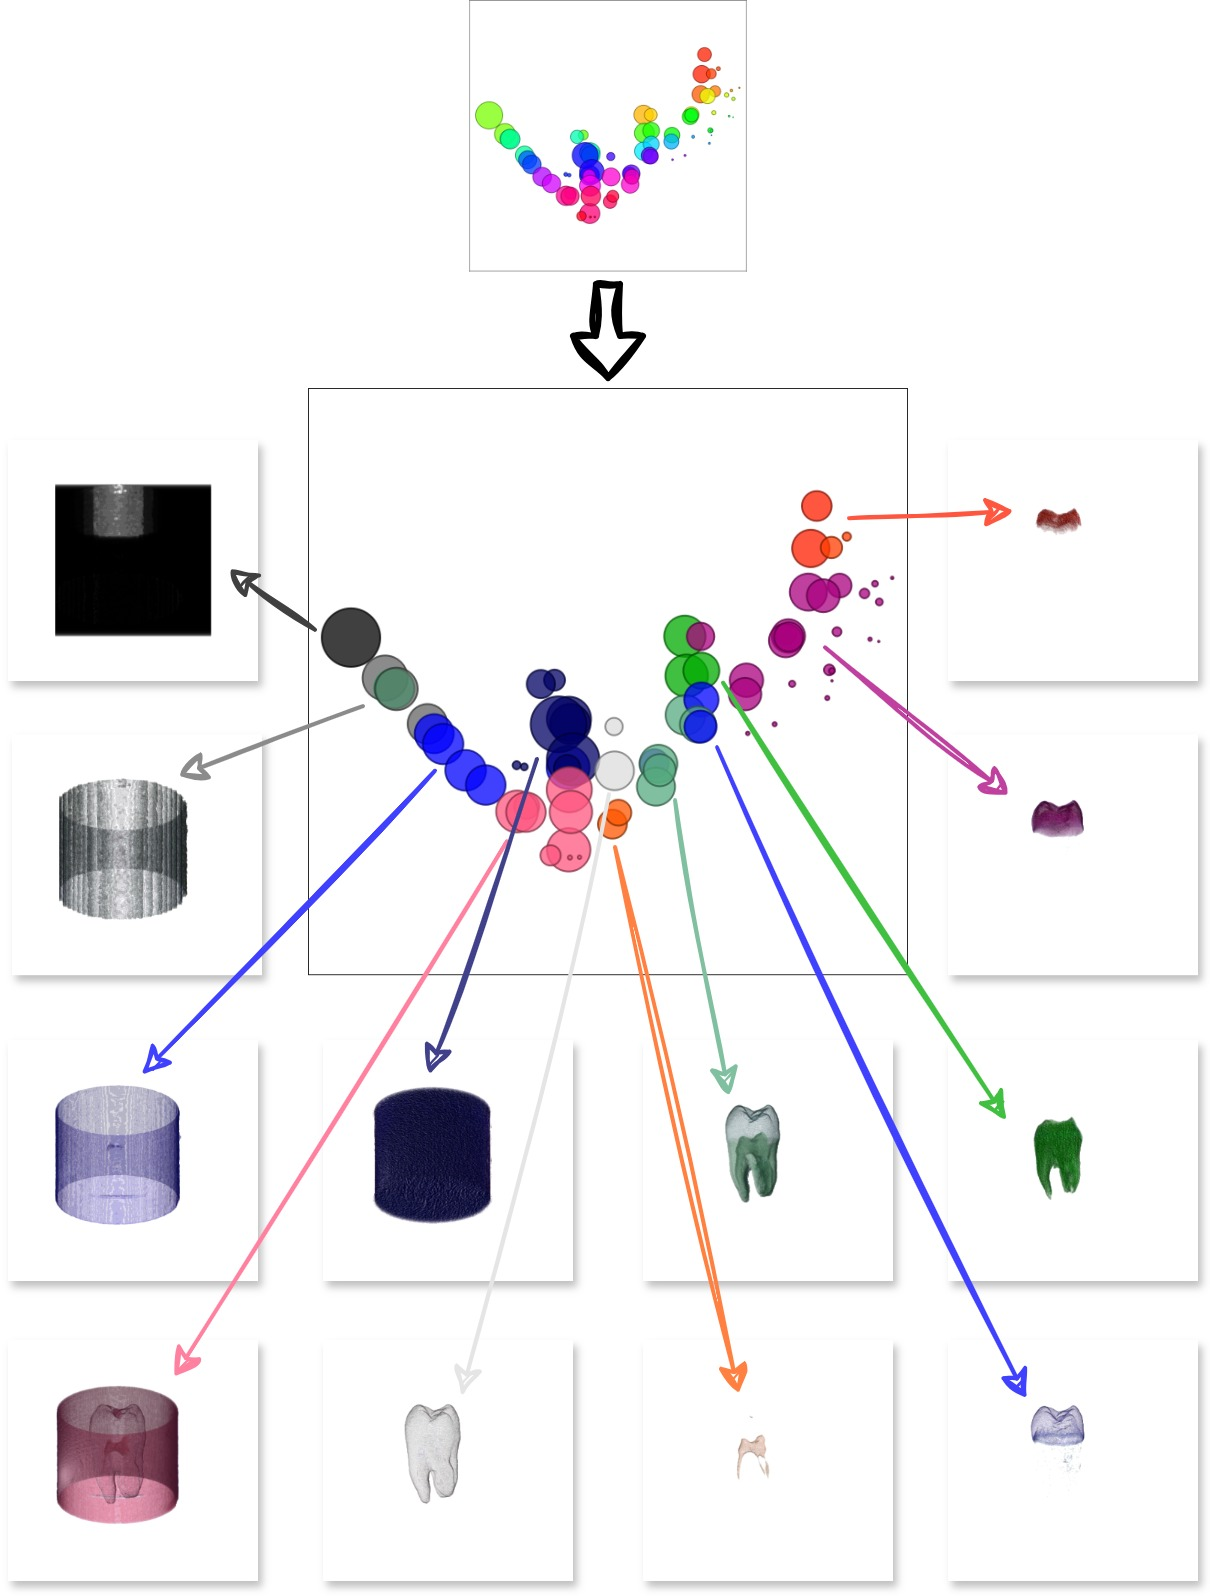
\includegraphics[width=\columnwidth]{figs/tooth-groups.jpg}
    \caption{Visual analysis of user-refined transfer function design and volume classification for tooth dataset. The volume details are manually grouped from an empirical perspective. The method parameters are set as follows: transfer function domain $ =\{$intensity, variance, absolute deviation, energy, contrast and entropy$\}$; $minPts = 4$; $\varepsilon = 0.23$; and $\alpha = 0.9$.}
    \label{fig:tooth-groups}
\end{figure}
%\section{Discussion}
\label{sect:discussion}

The two-level dimensionality reduction strategy effectively addresses challenges inherent in TFs. The first level offers guidance for TF definition, departing from the conventional approach reliant solely on user domain knowledge. This departure represents a significant advancement in the field. The second level simplifies the design interface.

While the feature selection heuristic shows promise in all experiments, the task ultimately remains the user's responsibility, which is a major limitation of our work. Investigating other unsupervised feature selection stop criteria may yield proper results, but there is a lack of investigation of these approaches in the TF context, warranting separate consideration in future analyses.

The parameters of DBSCAN significantly influence data classification. The parameter $minPts$ can assume a default value, $minPts = 4$~\cite{ester1996} since FastMap projects the data in a 2D space. The parameter 
$\varepsilon$ requires a fine-tune adjustment, but its behavior is stable. Higher values of $\varepsilon$ lead to fewer but larger clusters, while lower values increase the number of smaller clusters. 

Similarly, the adjustment of the SSS distance factor ($\alpha$) follows the same behavior, with $\alpha$ being inversely proportional to the number of pivots within each cluster.


The practical implementation of the method is supported by minimal computational overhead, indicating favorable scalability for large datasets in size aspect. Despite the computational expense of the feature selection step in higher-dimensional cases, the remaining method steps can handle it.
\section{Conclusions}
\label{sect:conclusions}

We presented a robust method for TF design that provides semi-automated feature classification and a simplified volume interaction space. Our method exhibits low computational overhead, as confirmed by short runtimes, highlighting its practicality and scalability for real-world applications.

Future work will focus on assessing the performance of the method with large, high-dimensional datasets to further validate its scalability and effectiveness.

Moreover, we aim to extend our evaluation to multivariate data, enhancing the applicability and robustness of the method across a wider range of volume datasets.

% \section*{Acknowledgements}
% This work was partially supported by the Brazilian Coordenação de Aperfeiçoamento de Pessoal de Nível Superior (CAPES). 

\section*{Declaration of Generative AI and AI-assisted technologies in the writing process}

During the preparation of this work the author(s) used ChatGPT 3.5 in order to improve readability and language of this paper. After using this tool/service, the author(s) reviewed and edited the content as needed and take(s) full responsibility for the content of the publication.





% trigger a \newpage just before the given reference
% number - used to balance the columns on the last page
% adjust value as needed - may need to be readjusted if
% the document is modified later
%\IEEEtriggeratref{8}
% The "triggered" command can be changed if desired:
%\IEEEtriggercmd{\enlargethispage{-5in}}

% references section

% can use a bibliography generated by BibTeX as a .bbl file
% BibTeX documentation can be easily obtained at:
% http://mirror.ctan.org/biblio/bibtex/contrib/doc/
% The IEEEtran BibTeX style support page is at:
% http://www.michaelshell.org/tex/ieeetran/bibtex/
\bibliographystyle{IEEEtran}
% argument is your BibTeX string definitions and bibliography database(s)
\bibliography{refs}
%
% <OR> manually copy in the resultant .bbl file
% set second argument of \begin to the number of references
% (used to reserve space for the reference number labels box)
%\begin{thebibliography}{1}
%
%\bibitem{IEEEhowto:kopka}
%H.~Kopka and P.~W. Daly, \emph{A Guide to \LaTeX}, 3rd~ed.\hskip 1em plus
%  0.5em minus 0.4em\relax Harlow, England: Addison-Wesley, 1999.

%\end{thebibliography}




% that's all folks
\end{document}


